% !TeX document-id = {a6531e15-bfcb-420a-930d-98791841ebe1}
% !TEX TS-program = xelatex
% !BIB program = biber
% !TEX encoding = UTF-8 Unicode

% 使用手冊請見 TW_Thesis_Template wiki:
% https://github.com/sppmg/TW_Thesis_Template/wiki

% User guide in wiki of TW_Thesis_Template :
% https://github.com/sppmg/TW_Thesis_Template/wiki

\documentclass[]{NTHU_thesis} % \documentclass[option1, option2, ...]
% Helpful options: 
% draft = Don't load figure ,reduce compile time.
% showframe = show document margins.
% colorgrid = show colored coordinate. (by eso-pic pkg.)
\usepackage[subpreambles]{standalone} % standalone class setting in config.tex
% Option ``subpreambles'' enable sub-tex's preambles when compile main tex. (pkg default disable)
% sppmg think it's still some problem (e.g. \addbibresource will faild ), recommend move all subpreambles to ``macros_preamble.tex``

\usepackage{slashed}

\begin{document}
    \frontmatter
        \startWatermark         % 由此開始每頁浮水印
        \documentclass[class=NTHU_thesis, crop=false, float=true]{standalone}
\begin{document}
% I use LaTeX3 to automatically generate name table. 
% Below \ExplSyntaxOn to \ExplSyntaxOff perpare prof. table contents,
% it will save contents to `\profsTableContent''. 
% You can ignore this block even you want make table by yourself.
\ExplSyntaxOn
% Copy prof. list from config.tex
\clist_gclear_new:N \g_sppmg_profsZh_cl
\clist_gset:NV \g_sppmg_profsZh_cl \profsZh
\clist_gclear_new:N \g_sppmg_profsEn_cl
\clist_gset:NV \g_sppmg_profsEn_cl \profsEn

% get total number of prof. . Omitted language will not display.
\int_gzero_new:N \g_sppmg_profTotal_int
\int_gset:Nn \g_sppmg_profTotal_int {
    \int_max:nn {\clist_count:N \g_sppmg_profsZh_cl} 
        {\clist_count:N \g_sppmg_profsEn_cl}
}

% NOTE: ``tabularx'' will  processes its contents more than once 
% for calculate width, so ``gpop'' can't put in tabularx env.
% \tl_if_exist:NTF {\tl_clear:N \g_sppmg_tableContent_tl} {\tl_new:N \g_sppmg_tableContent_tl}
% \tl_if_exist:NTF \g_sppmg_tableContent_tl {} {\tl_new:N \g_sppmg_tableContent_tl}
\tl_gclear_new:N \g_sppmg_tableContent_tl


% Use a inline function for pop 2 list (zh+en), and save table content 
% Input(#1) switch 3 case, 1 = Advisor, 2 = committee member , 3+ is more.
% Use ``for'' loop to get all prof.
\int_step_inline:nnnn {1}{1}{\g_sppmg_profTotal_int}{
    \clist_gpop:NNTF \g_sppmg_profsZh_cl \l_tmpa_tl {}{ \tl_clear:N \l_tmpa_tl}
    \clist_gpop:NNTF \g_sppmg_profsEn_cl \l_tmpb_tl {}{ \tl_clear:N \l_tmpb_tl}
    \tl_gput_right:Nx \g_sppmg_tableContent_tl {
        \int_case:nnTF {#1}{
            {1} {指導教授: & \l_tmpa_tl & 博士 & (Prof.~ \l_tmpb_tl ) \exp_not:n {\\} }
            {2} {共同指導: & \l_tmpa_tl & 博士 & (Prof.~ \l_tmpb_tl ) \exp_not:n {\\} }
        }{}{
            & \l_tmpa_tl & 博士 & (Prof.~ \l_tmpb_tl ) \exp_not:n {\\} 
        }
    }
}

% Copy contents to LaTeX2e macro.
\cs_set_eq:NN \profsTableContent \g_sppmg_tableContent_tl

\ExplSyntaxOff
\def\fsUniversity{\fs{24}[1.5]}
\def\fsTitle{\fs{20}[1.5]}
\def\fsNames{\fs{18}[1.5]}

\def\mcShift{\hspace{-6.0pt}} % It's for align non-multicolumn cell .
% --------define title page layout for thesis
\titlepageFontFamily % set in config.tex
\newgeometry{top=2.5cm, bottom=2.5cm, inner=2cm, outer=2cm} % only for titlepage
\begin{spacing}{1.0}
\begin{titlepage}
    \null\vfill
    \begin{center}
        {\fsUniversity 國\quad 立\quad 清\quad 華\quad 大\quad 學} \par
        \vspace*{5mm}
        
        {\fsTitle {\degree}論文\par}
        \vspace*{20mm}
        
        {\fsTitle {\title} \par}
        \vspace*{5mm}
        
        {\fsTitle {\subtitle} \par}
        \vspace*{10mm}
        
        {\ifx \logo\empty\vspace*{30mm}
        \else \includegraphics[height=30mm]{\logo} \par
        \fi}
        \vfill
        
        {\fsNames \renewcommand{\arraystretch}{1}
            % If you want make table by yourself, replace ``\profsTableContent''
            \begin{tabular}{l@{\hspace*{0.4em}}l@{\quad}l@{\quad}l}
            系\qquad 所: & \multicolumn{3}{l}{\mcShift \dept}      \\
            學\qquad 號: & \multicolumn{3}{l}{\mcShift \studentID} \\
            研\enspace 究\enspace 生: & \authorZh & & (\authorEn)    \\
            
            \profsTableContent
            
            \end{tabular}
        \par}
        \vspace*{5ex}
        
        {\fsTitle {\degreedate} \par}
        \vspace*{2ex}
        
        \ifthenelse{\boolean{printcopyright}}
        {{{版權所有\copyright\ \author\ \quad \copyyear} \par}}
        {}
    \end{center}
    \null\vfill
\end{titlepage}
\end{spacing}
\restoregeometry
\normalfont % use main font
%--------end of title page for thesis
\cleardoublepage
\end{document}
       % 封面/書名頁
        \listoftodos   % todo list, hide when set \textbackslash{}setboolean\{publish\}\{\textbf{true}\} in config.tex. It will not add to TOC , you can add \todototoc before \listoftodos to do that.
            \todo[inline]{``Todo List'' will hide when set \textbackslash{}setboolean\{publish\}\{\emph{true}\} in config.tex.}

        %%%%%%%%%%%% letters %%%%%%%%%%%%
        % Set file name in config.tex
        % 依校方規定,此處須插入:
        % [v] 清大(電子授權書) 必備,不論是否授權都要裝訂
        % [v] 清大(紙本授權書) 必備,不論是否授權都要裝訂
        % [x] 國家圖書館(電子授權書) 有授權才要裝訂
        % [v] 國家圖書館(紙本論文延後公開/下架申請書)→紙本論文有申請延後公開才要裝訂
        % [v] 指導教授推薦書
        % [v] 考試委員審定書
        % !!! [x] 部份請自行插入

        % 碩博士論文電子檔授權書 Authorization Letter (for electronic)
        \IfFileExists{\letterAuthEl}{
            \cleardoublepage        % 由下個右頁開始
            \includepdf{\letterAuthEl}}{}
        % 碩博士論文紙本授權書 Authorization Letter (for paper)
        \IfFileExists{\letterAuthPa}{
            \cleardoublepage        % 由下個右頁開始
            \includepdf{\letterAuthPa}}{}
        % 國家圖書館(電子授權書) 有授權才要裝訂

        % 碩博士紙本論文延後公開/下架申請書。(如需延後公開者,才需要裝訂於論文內頁)
        \IfFileExists{\letterPubReq}{
            \cleardoublepage
            \includepdf{\letterPubReq}}{}
        % 指導教授推薦書
        \IfFileExists{\letterRecom}{
            \cleardoublepage
            \includepdf{\letterRecom}}{}
        % 口試委員審定書
        \IfFileExists{\letterVerif}{
            \cleardoublepage
            \includepdf{\letterVerif}}{}
        \cleardoublepage
        
        %%%%%%%%%%%% Other frontmatter, eg,abstract %%%%%%%%%%%%
        % 中英文論文摘要:內容應說明研究目的,資料來源,研究方法及研究結果等
        \documentclass[class=NCU_thesis, crop=false]{standalone}
\begin{document}
\setlength{\parindent}{2em} %縮排2字寬

\chapter{摘要}
	我們透過大強子對撞機中的ATLAS探測器量測與一般物質有交互作用的物質的特性,分析某模型預測中,較不能與一般物質有交互作用之物質的存在與否,對於其背景事件的研究將在本篇文章中提及。

\vspace{2em}

\noindent \textbf{關鍵字:} \keywordsZh{} % Set keywords in config.tex
\end{document} % zh 中文摘要
        \documentclass[class=NCU_thesis, crop=false]{standalone}
\begin{document}

\chapter{Abstract}
Write your English abstract here.



\vspace{2em}
\noindent \textbf{Keywords:} \keywordsEn{} % Set keywords in config.tex
\end{document} % en 英文摘要
        \documentclass[class=NCU_thesis, crop=false]{standalone}
\begin{document}

\chapter{Acknowledgement}

首先,我要先感謝我的指導教授,徐百嫻老師。感謝她自我大學三年級始從零開始教導我在這方面的知識與研究態度,也是她在我對於研究內容迷茫時給予我建議與指點。

其次,我也要感謝此次研究的主要領導人,University of Washington的Samuel Meehan博士後研究員、Max-Planck-Institut f\"{u}r Physik的Patrick Reick博士後研究員、Nikhef and Radboud University的Frank Filthaunt教授與University of Washington的Shih-Chieh Hsu教授,感謝他們對於我們的研究提出討論的與統籌。

也感謝Ludwig-Maximilians-Universit\"{a}t M\"{u}nchen的Andrea Matic博士生,她在我剛進到分析團隊時對於我在分析程式理解上有著非常大的幫助。

另外,我也必須感謝呂昀儒博士後研究員,是他提供了在技術上碰到的疑難雜症的處理方式與提供更快速,以及更有系統性的分析方式。

除此之外,也對自己研究上的夥伴,施柏杉同學以及詹予欣學妹在討論上提供的一切幫助,使我能夠透過討論吸取更多知識與處事方法等。

更要銘謝蔡孟儒學弟,雖然其分析的範疇與此有一些差異,但還是願意與我討論我可能碰到的問題,並也提出各種有實質可能性上的建議。

還要對於在分析團隊上對彼此分析有幫助的每一位成員做出最大的感謝,是大家一起的努力才能完成此次的分析成果。

最後,還要感謝所有在背後支持我的人。研究室的羅令崴博士後研究員、簡上淯博士生、李俊豪博士生、葉書瑋博士生、陳祐君碩士、盧致融碩士生、王斌碩士生,謝謝他們的陪伴,能在研究遭遇瓶頸之際給予適當歡笑與慰藉。也感謝象棋社的楊宗諭老師、朱緯東學長、郭達毅學長、許浩哲學弟、楊上民學弟、陳其伸學弟能讓我在每週有短暫的時光得以釋放壓力。更感謝在研究之餘參與助教工作認識的詹貴麟博士生與孫乙立碩士,謝謝你們經常與我交換研究生涯碰到的意見。

要感謝的人不僅止於此,筆者一併在此再一由衷感謝,未能盡到周詳提及之處,尚且包涵。

\end{document}


 % 誌謝(可略)

        % 原始 book class 不將 TOC,LOF,LOT 加入目錄列表,須手動加
        % 此樣板可由 config.tex 切換是否自動加入目錄
        \tableofcontents        % 目錄
        \listoffigures          % 圖目錄
        \listoftables           % 表目錄
        \documentclass[class=NCU_thesis, crop=false]{standalone}
\begin{document}

\chapter{Glossary}
Use table for symbol list. You can also use package ``nomencl'' (simple) or ``glossaries'' (powerful). see packages document or my tutorial (but it's Chinese).

\begin{table}[h]
    \normalsize
    \centering
    \begin{tabular}{c@{\quad:\quad}l}
%         Symbol  & Description \\ 
        VIM     & The best guy's editor \\ 
        Emacs   & The God's editor \\ 
        CTAN    & Comprehensive TeX Archive Network, ctan.org \\
        
    \end{tabular} 
    \caption*{Glossary} % Hide caption by comment/remove it, label will inactive also. 不想顯示請註解/刪除\caption行(\label自動失效)
    \label{table:glossary_def}
\end{table}

\end{document}
    % 符號說明
    \mainmatter
        \documentclass[class=NCU_thesis, crop=false]{standalone}
\begin{document}
	
	
\chapter{Introduction}
	It is generally acknowledged that the universe does not only contain matter. Dark matter (DM) \cite{hep-ph/0404175} comprises more percentage in the universe than matter, and its nature remains one of the biggest unknown question in physics. A striking hypothesis on the nature of DM \cite{STEIGMAN1985375, PhysRevD.33.1585} is that it is a electrically neutral, and thus being dark, stable particle, denoted as $\chi$. It has weak interactions with Standard Model (SM) particles in addition to gravitational interactions. Its mass is predicted be to range from the order of GeV to TeV. In this hypothesis, ways of its detection are presented and carried out as shown in figure \ref{fig:DM search}. A collider way of detection for the DM \cite{1507.00966} is discussed in this thesis.
	
	\fig[0.4][fig:DM search][!hbt]{DM_search.png}[Different ways of dark matter search. Studies on the SM particles that are predicted to be the products of DM interactions are the indirect search. Researches on the SM particles which are assumed to have interaction with DM are the direct way of search. Colliding the SM particles and investigating the undetected parts of the products is the collider way of detection.][short caption]
	
	\newpage
	
	The DM signature in the collider under the hypothesis that they weakly interact with SM particles is the missing momentum. It can be observed by a detectable particle \textit{X} that produced in associated with the DM. Such \textit{X}+missing momentum signature is explored by the LHC (Large Hadron Collider) experiments with \textit{X} being a jet (would be discussed in section \ref{jet}) \cite{1711.03301, 1712.02345}, a heavy quark \cite{1710.11412, 1711.11520, 1801.08427, 1706.02581}, a vector boson \cite{1712.02345, 1704.03848, 1708.09624, 1711.00431, 1706.03794, 1701.02042}, or a Higgs boson \cite{1706.03948, 1707.01302, 1806.04771, 1703.05236}. This thesis presents the search with \textit{X} being a Higgs boson \textit{h} that further decays into a pair of b-quarks, $h \rightarrow b\bar{b}$, which is the most frequent decay channel of \textit{h}. The analyzed dataset of proton-proton collisions has the center-of-mass energy $\sqrt{s} = 13$ TeV and was recorded by ATLAS (\textbf{A} \textbf{T}oroidal \textbf{L}HC \textbf{A}pparatu\textbf{S}, would be discussed in chapter \ref{ATLAS}) during 2015 to 2017, corresponding to an integrated luminosity of 79.8 $fb^{-1}$.
	
	Another progress in this analysis is the introduction of variable-radius jet, which would result in improvements in object reconstruction and performance. More information would be discussed in section \ref{VR jets} and its effect compared to the previous iteration is covered in chapter \ref{result}.
	
	\fig[0.4][fig:zp2HDM][!hbt]{zp2HDM.png}[The Feynman diagram of the $Z'$-2HDM model in leading order. The collison of two SM particles produces the mediator $Z'$, which further decays into a SM Higgs \textit{h} and a pseudo-scalar Higgs \textit{A}. The pseudo-scalar Higgs \textit{A} is assumed to decay into a pair of DM candidate particles. The decay channel of the SM Higgs is a pair of b-quarks for this analysis.][short caption]
	
	The siganl model used in this iteration is a Type-II two-Higgs-doublet model (2HDM) \cite{1707.01302} with an additional mediator $Z'$, which is referred to as the $Z'$-2HDM model. In the siganl model, one scalar Higgs boson \textit{h} and a pseudo-scalar Higgs \textit{A} are found. The whole process reads $pp \rightarrow Z' \rightarrow Ah \rightarrow \chi \bar{\chi} b \bar{b}$, in which the DM pair decay from \textit{A} and the b-quarks pair decay from \textit{h}. The Feynman diagram is shown in figure \ref{fig:zp2HDM}. The relevant parameters are the masses $m_{\mathrm{A}}$, $m_{\mathrm{Z'}}$, $m_{\chi}$, the coupling of $Z'$, $g_{Z'}$ and $\tan(\beta)$, the ratio of the vacuum expectation values of the two Higgs fields coupling to up-type and down-type quarks.
	
	The main SM backgrounds are the top-quark pairs ($t\bar{t}$) and vector bosons (\textit{W} or \textit{Z} boson) with b-jets. The signal region and control region are used to constrain the background. More details would be covered in chapter \ref{Event selection}.
	
\end{document}    % 緒論
        \documentclass[class=NCU_thesis, crop=false]{standalone}
\begin{document}

\chapter{The ATLAS detector}
\section{Coordinates}
	The ATLAS (\textbf{A} \textbf{T}oroidal \textbf{L}HC \textbf{A}pparatu\textbf{S}) experiment is one of the seven detector in Large Hadron Collider (LHC) at CERN (European Organization for Nuclear Research). Its cylindrical symmetry and end caps covers nearly $4\pi$ in solid angle.
	
	A coordinate system is used to describe every location near ATLAS. The origin is set at the center of the detector, or the interaction point. The x-axis points toward the center of the LHC ring; the y-axis points vertically upward; the z-axis points along one of the beam pipe direction such that a right-handed coordinate sysetem is created.
	
	A modified version of cylindrical coordinate is more commonly used in the experiment. The pseudorapidity $\eta \equiv -\ln\tan(\theta / 2)$, in which $\theta$ is the polar angle in cylindrical coordinate, is used to decribe the angle between the z-axis and the direction of interest. $(r, \phi)$ is the same system to describe the tranverse plane, with $\phi$ being the azimuthal angle. In addition, the cone size is defined as $\Delta R \equiv \sqrt{(\Delta \phi)^2 + (\Delta \eta)^2}$.

\end{document}          % 分析方法
        \documentclass[class=NCU_thesis, crop=false]{standalone}
\begin{document}

\chapter{Object Selection and Reconstruction}
	Signals recorded in the ATLAS detector are categorized or reconstructed as pysical objects, which could be further used in the analyses. Besides the head-to-head, or hard-scattered, events which have high transverse momentum, or $p_T$, there are also additional collisions with lower $p_T$. These are referred to as the pile-up events, which one often wants to exclude in the analyes. The reconstruction and definition of objects used in this study are listed in the following.
	
\section{Jets}
	Jets are the reconstruction of collimated bunches of hadrons. In ATLAS experiment, the anti-$k_T$ algorithm is usually used to recombine hadrons into cone-sized shapes. In short, the anti-$k_T$ algorithm makes use of $p_T$ of each given entities and reconstructs jets whose R is the given radius parameter and which center on hard-scattered particles. How the jets is reconstructed and defined in this study is tabulated in table.\ref{tab:jet selection} and explained as follows.
	
	\begin{table}[h]
		\centering
		\caption{The summarization of the jet selection and reconstruction.}
		\label{tab:jet selection}
		\begin{tabular}{|c|c|c|c|c|}
			\hline
			type & \shortstack{(\textit{central})\\small-R jets} & \shortstack{(\textit{forward})\\small-R jets} & large-R jets & VR track jets \\ \hline
			$p_T$ (GeV) & > 20 & > 30 & > 200 & > 0.5 \\ \hline
			$\lvert \eta \rvert$ & (0, 2.5) & (2.5, 4.5) & (0, 2.0) & (0, 2.5) \\ \hline
			$R$ & \multicolumn{2}{c|}{0.4} & 1.0 & \shortstack{$p_T / \rho \in$ (0.02, 0.4)\\ with $\rho = 30$ GeV} \\ \hline
			additional & \shortstack{if $\lvert \eta \rvert < 2.4$ then\\$p_T < 60$ GeV} & \multicolumn{2}{c|}{-} & $\lvert z_0 \sin(\theta) \rvert < 3$ mm \\ \hline
		\end{tabular}
	\end{table}
	
	\subsection{Small-radius Jets}
		Using the anti-$k_T$ algorithm with a raidus parameter of 0.4, small-radius, or small-R, jets can be reconstructed from the energy deposits in the calorimeter. Small-R jets are further categorzied into two types, the central jets and the forward jets. Those jets whose $\lvert \eta \rvert < 2.5$ are required to have $p_T > 20$ GeV in order to be identified as the former; other jets with $2.5 < \lvert \eta \rvert < 4.5$ are referred to as the latter and a threshold of $p_T > 30$ GeV is required. For jets in $\lvert \eta \rvert < 2.4$, an additional threshold of $p_T < 60$ GeV is required, and, to further suppress jets from the pile-up interactions, they are required to be originated from the reconstructed location of the collision, or the primary vertex.
	
	\subsection{Large-radius Jets}
		The large-radius, or large-R, jets are reconstructed via the anti-$k_T$ algorithm with a radius parameter of 1.0. The reconstruction highly depends on the calorimeter and the tracking system. Certain calibration method is appiled for the energy deposits in the calorimeter. The calibrated jets have a $p_T$ threshold of 200 GeV and are required to be within the range of $\lvert \eta \rvert < 2.0$.
	
	\subsection{Variable-radius Jets}
		The variable-radius (VR) track jets are also reconstructed using the anti-$k_T$ algorithm. Those jets whose $p_T$ does not exceed 0.5 GeV or out of the range of $\lvert \eta \rvert < 2.5$ are not considered. To suppress the pile-up jets, a creiteria on the longitudinal impact parameter, $\lvert z_0 \sin(\theta) \rvert < 3$ mm, is required, where $z_0$ is the point closet to the vertex along the logitudinal axis and $\theta$ is the polar angle of the track. The main feature of the VR track jets is that the radius parameter depends on the value of $p_T$ rather than a constant value:
		\begin{equation}
			R \rightarrow R_{\mathrm{eff}} \approx \frac{p_T}{\rho},
		\end{equation}
		in which $\rho$ is set at 30 GeV, which is the optimal value ragarding the efficiency for b-tagging. The upper limit and lower limit, $R_{\mathrm{max}}$ and $R_{\mathrm{min}}$ are set at 0.4 and 0.02 in this regard.
	
\section{Leptons}
	Leptons are used to categorized the regions selected in this analysis, which would be covered in the next chapter. Requirements of each flavor are explained in the following and summarized in table.\ref{tab:lepton selection}.
	
	\begin{table}[h]
	%\centering
	\caption{The summarization of lepton selection and reconstruction. The rightmost column are the requirements for the reconstructed small-R jet that decays from a $\tau$-lepton candidate.}
	\label{tab:lepton selection}		\begin{tabular}{|c|c|c|c|c|c|}
		\hline
		flavor & \multicolumn{2}{c|}{e} & \multicolumn{2}{c|}{$\mu$} & $\tau$ \\ \hline
		categorization & baseline & signal & baseline & signal & - \\ \hline
		$p_T$ (GeV) & > 7 & > 27 & > 7 & > 25 & > 20 \\ \hline
		$\lvert \eta \rvert$ & \multicolumn{2}{c|}{(0, 2.47)} & (0, 2.7) & (0, 2.5) & (0, 1.37) $\cup$ (1.52, 2.5) \\ \hline
		ID & \multicolumn{2}{c|}{Loose} & \multicolumn{2}{c|}{\shortstack{Loose (0/2-muon)\\ Medium (1-muon)}} & Loose \\ \hline
		transverse impact parameter & \multicolumn{2}{c|}{$d_0 / \sigma(d_0) < 5$} & \multicolumn{2}{c|}{$d_0 / \sigma(d_0) < 3$} & $\lvert d_0 \rvert < 1$ mm \\ \hline
		$\lvert z_0 \sin(\theta) \rvert$ (mm) & \multicolumn{4}{c|}{< 0.5} & < 1.5 \\ \hline
		Additional & \multicolumn{4}{c|}{-} & \shortstack{one to four track-jets\\$\Delta \phi(\tau, \slashed{E}_T) < \frac{\pi}{8}$}\\ \hline
		\end{tabular}
	\end{table}

	\subsection{Electrons}
		Electron candidates are reconstructed from the energy deposits in EM calorimeter that match a track recorded in the inner detector. In addition, there is a LLH-based algorithm, which further makes use of multivariable analysis (MVA), applied for the electron ID. Three levels of ID operating point, loose, medium and tight, are povided; among them, loose ID is used in this study for the electrons. Moreover, electrons are divided into two groups, the baseline electrons, whose $p_T$ exceed 7 GeV, and the signal electrons, which requires a tighter threshold of $p_T > 27$ GeV. All candidates within $\lvert \eta \rvert < 2.47$ are considered. Finally, requirements of the impact parameter are considered, both in the transverse and logitudinal directions. For the former, the relative resolution, which is the fraction of the transverse impact parameter $d_0$ and its resolution $\sigma(d_0)$, has an upper bound of 5. For the latter, the value $\lvert z_0 \sin(\theta) \rvert < 0.5$ mm is set.
		
	\subsection{Muons}
		Muon candidates, also divided into baseline and signal muons, are reconstructed with high dependence of inner detector and the muon spectrometer. Signal muons, whose $p_T$ exceed 27 Gev, are more likely to leave tracks in the inner detector, and thus shall be found in $\lvert \eta \rvert < 2.5$. For baseline muons, which have a looser $p_T$ threshold of 7 GeV, leaving signals in the inner detector is not required and thus are within $\lvert \eta \rvert < 2.7$, which is the range of the muon spectrometer. On top of that, the impact parameter must be consistent with the the primary vertex. $d_0 / \sigma(d_0) < 3$ and $\lvert z_0 \sin(\theta) \rvert < 0.5$ mm are set. Finally, a loose ID is used for the zero-lepton and two-muon channel whilst the one-muon channel makes use of a medium ID for the muons in this analysis. These channels would be covered in the upcoming chapter.
		
	\subsection{Taus}
		$\tau$-leptons, whose decay length is few $\mu$m, barely reach the ATLAS detector and thus are mainly reconstructed from their decay products. Due to the fact that most of the $\tau$-leptons decay into hadrons, the $\tau$-lepton candidates are reconstructed from jets. The transverse impact parameter, $\lvert d_0 \rvert < 1$ mm, and the logitudinal one, $\lvert z_0 \sin(\theta) \rvert < 1.5$ mm, are set for the jet tracks and the $\tau$ vertex. The threshold on the $p_T$ of the jets is set at 20 GeV; the range of $\lvert \eta \rvert < 2.5$, excluding $1.37 < \lvert \eta \rvert < 1.52$, which is the region between the barrel and the forward region, or the crack region, is also required. Furthermore, the ID is built on a boosted decision tree (BDT) that makes use of the information from the tracks and the calorimeter. The loose working point on the $\tau$-leptons is used. Finally, the small-R jet is required to contain one to four track-jets and within a range of $\Delta \phi < \frac{\pi}{8}$ with the missing transverse energy (MET, $E_T^{\mathrm{miss}}$ or $\slashed{E}_T$) in order to suppress the W-boson-decayed $\tau$-leptons.
	
\section{Missing Transverse Momentum}
	The missing transverse momentum is the imbalance in $p_T$ of the reconstructed objects. Thus, it can be reconstructed as the negative vector transverse momentum sum. This includes the hard-scattered objects and the soft term. The momentum of hard-scattered reconstructed particles construct the former. As for the soft term, tracks that are not associated to any reconstructed hard objects are considered. The vetoed leptons, which are the leptons that needs to removed from the analysis in some scenario and would be covered in the next chapter, also count as the soft term. Jets that failed the selection of small-R jets also contributes the soft term, with the $p_T$ threshold on the forward jet being modified to 20 GeV. The value of the missing transverse momentum is denoted as $E_T^{\mathrm{miss}}$ (or $\slashed{E}_T$).
	
	An estimation variable $E_T^{\mathrm{miss}}$ significance, S, is used to check the genuinity in whether the $E_T^{\mathrm{miss}}$ comes from undectable particles instead of mismeasurements or any inefficiencies.
	
\section{Overlap Removal}
	Object ambiguities happen when objects match multiple reconstruction criteria. In the following listed specific steps of object reconstruction that is require to solve the problem.
	\begin{enumerate}
		\item If two electron candidates share the same track, remove the one with lower $p_T$.
		\item If a $\tau$-lepton candidate lies within $\Delta R = 0.2$ of an electron or muon, it is removed.
		\item Reject the electron candidates whose track is shared with a muon candidate.
		\item Small-R jets are removed if they are within $\Delta R = 0.2$ of an electron.
		\item Remove the electrons that are within $\Delta R = \min(0.4, 0.04 + 10 GeV / p_T^{\mathrm{electron}})$ of a small-R jet.
		\item If the separation between a small-R jet and a muon is within $\Delta R = 0.2$, the small-R jet is removed provided that it has fewer than three tracks or that the muon $p_T$ is greater than 50\% of the jet $p_T$ and is greater than 70\% of the $p_T$ sum of the tracks associated to the jets.
		\item Remove the muons that are within $\Delta R = \min(0.4, 0.04 + 10 GeV / p_T^{\mathrm{muon}})$ of a small-R jet.
		\item Large-R jets whose track is within $\Delta R = 0.1$ to that of an electron are removed.
	\end{enumerate}

\end{document}          % 實驗結果
        \documentclass[class=NCU_thesis, crop=false]{standalone}
\begin{document}

\chapter{Event Selection}
This is the start of the event selection.

\fig[0.4][fig:zp2HDM][!hbt]{zp2HDM.png}[Test][short caption]

\end{document}      % 結論
        \documentclass[class=NCU_thesis, crop=false]{standalone}
\begin{document}

\chapter{Study on the Background Estimation}
	As mentioned in the last chapter, the CRs are used to estimate the backgrounds in the SR. Because W+jets events and $t\bar{t}$ events in both SR and one-muon CR are the same processes, one assumes the kinematics are the same. As for the two-lepton CR, first note that the mass of the charged leptons and neutrinos are negligible compared to that of the Z boson. Thus, one can argue that the kinematics of the Z(ll)+jets and Z($\nu \nu$)+jets events are roughly the same, where the Z(ll) means the charged-leptonic decay of the Z boson.
	
	During the analysis, the author and Po-Shan Shih, partner of the author, are both working on the estimation of the two-lepton CR. In this chapter, the problems that the author participated or fixed during the study are stated. Also, a shape difference of W($\mu \nu$)+jets events in SR and one-muon CR is carried out as an additional work.
	
	\section{Overlap Removal}
		The comparison plots of Monte Carlo (MC) to data are always reviewed by analyzers. Those plots are referred to as the pre-fit plots. The pre-fit plots contain the data and MC samples that pass the selection criteria. Those events are then filled in the plot based on the value of the physical quantity of interest.
		
		An unusual peak was spotted in one of the Z+jets CR plot during the analysis, as shown in figure \ref{fig:OR_before}. The plot is the distribution of the leading large-R jet mass and the peak is within 90 to 105 GeV. It is unusual because the statistics of the mass spectum should generally become less as the energy goes up. However, the peak reveals that many events assemble around a high energy value and thus creates a discontinuity.
		
		\fig[0.5][fig:OR_before][!hbt]{OR_before.png}[The plot which shows the issue of overlap removal. It shows the distribution of leading large-R jet mass. The dotted points represent the data while the solid histogram shows the MC simulations. Both of them pass the selection criteria of two-lepton CR. The spotted unusual peak lies in the bin of 90 to 105 GeV. The legends of "Z+mumu" and "Z+ee" in the upper-right of the plots are typos which weren't fixed at that time. They refer to the MC simulations of Z(ee)+jets and Z($\mu \mu$)+jets events respectively.][short caption]
		
		The bin includes the Z boson mass, which is about 91 GeV. From the Feynman diagram of the Z+jets background (figure \ref{fig:subfig_Zjets}) with the neutrinos replaced with leptons, one can tell that the invariant mass of the lepton pair would be close to that of a Z boson. In figure \ref{fig:OR_before}, nevertheless, it is large-R jet that has the invariant mass around it.

		Because all these events pass the two-lepton CR selections as stated in section \ref{2LCR}, one of the possible explanation to this peak is misidentification of leptons and large-R jets. It happens when they share the same track or overlap. From figure \ref{fig:OR_before}, one recognizes that the Z(ee)+jets events contributes the most in that bin. Recall the last reconstruction strategy from section \ref{OR} that an electron is removed if it it within $\Delta R = 0.1$ with a large-R jet.
		
		As a result, a check in the codes on the overlap removal (OR) was conducted, and the same plot after adding it is shown in figure \ref{fig:OR_after}. From the plot, one can see that the peak around the Z boson mass is removed. This discovery and study reveal the fact that OR wasn't properly applied at that time. After a careful check on the codes with the developer of the framework we used, the OR problem was officailly fixed.
		
		\fig[0.5][fig:OR_after][!hbt]{OR_after.png}[The plot which shows the result after overlap removal applies properly. The dotted points represent the data while the solid histogram shows the MC simulations.][short caption]
	
	\section{Dealing with Large Weights}
		There are unexpected situation during real data collecting at the detector, which is not simulated by the MC. To further include these possibilities in the simulations, weights are applied. After the calculations done by MC, the raw number of events would be multiplied by these weights.
		
		Another peak was discovered in the Z+jets CR plot during the analysis, as shown in figure \ref{fig:unfixed posW}. The shown plot is also the distribution of leading large-R jet mass, but it also appeared in other different plots. Following the logic in the last section, one can tell that it is unusual. However, because of the fact that OR had fixed this time and also because of this spike-like behavior existed in other kinematic variable plots, it must be a result of a different issue.
		
		As it turned out, an event was multiplied by a really high generator weight which resulted in a large contribution to the MC. The reason of this is a result of a random generation, which happens in the the type of MC generator the analyzers used. Another similar weird behavior could happen when the generator weight is a great negative value, as shown in figure \ref{fig:unfixed negW}, which was another plot during the analysis. A clear pit shows up in the distribution where it should be continuous.
		
		\fig[0.6][fig:unfixed posW][!hbt]{unfixed_posW.jpg}[The plot which shows the unusual peak resulting from the generator weight. It shows the distribution of leading large-R jet mass. The dotted points represent the data while the solid histogram shows the MC simulations. The legends of "Z+mumu" and "Z+ee" in the upper-right of the plots are typos which weren't fixed at that time. They refer to the MC simulations of Z(ee)+jets and Z($\mu \mu$)+jets events respectively.][short caption]
		
		\fig[0.6][fig:fixed posW][!hbt]{fixed_posW.jpg}[The plot which shows the result after the event with large generator weight removed. Comparing to \ref{fig:unfixed posW} reveals that the peak disappears.][short caption]
		
		The solution to these weights in this iteration is to remove those events, because the number of events with these extreme value of generator weight is small and negligible. The results after removing the events are shown in figure \ref{fig:fixed posW} and \ref{fig:fixed negW}.
		
		\fig[0.6][fig:unfixed negW][!hbt]{unfixed_negW.pdf}[The plot which shows the unusual pit. It shows the distribution of dijet mass. The dotted points represent the data while the solid histogram shows the MC simulations.][short caption]
		
		\fig[0.6][fig:fixed negW][!hbt]{fixed_negW.pdf}[The plot which shows the result after the events with large negative value of generator weight are removed. Comparing to \ref{fig:unfixed negW} reveals that the pit disappears.][short caption]
	
	\section{W($\mu \nu$) +jets Events Shape Comparison}
		As mentioned in the beginning of this chapter, the W+jets and $t\bar{t}$ events in either SR or one-muon CR are assumed to have the same kinematics. Thus, one-muon CR can be made use of estimating the background in SR. However, the author wonders whether the comparison of the kinematics between these two regions matches. Therefore, a study on this is performed.
	
		A set of W($\mu \nu$)+jets Monte-Carlo (MC) samples is used. In these samples, the selection for one-muon CR and SR mentioned in the last chapter are applied. The samples after the selections of SR is used as a comparison to the one-muon CR.
		
		The reason why a comparison between W($\mu \nu$)+jets samples and data is not used is because one cannot know the truth-level comparison via it. The data after the one-muon selections would contain the $t\bar{t}$ events since they are also one of the estimation target of one-muon CR. If one adds the $t\bar{t}$ MC samples in the comparison, data and MC comparison is apple-to-apple, but one would lose the information of the shape difference on W($\mu \nu$)+jets events only. 

		Because one doesn't know the yields of both samples after the selection, a normalization is used on them. After normalization, one can deduce the shape difference without any adjustment on the yields of one of them. The events are put in a histogram plot for comparison. The shape comparison for (proxy) $E_T^{\mathrm{miss}}$ is shown in figure \ref{fig:MET_comparison}. Besides, a yields uncertainty of 5\% is assigned to this SR and one-muon CR extrapolation. The reason of 5\% is due to the fact that some uncertainties used in this analysis follow the results of another analysis group, the Vh(bb) group, including this uncertainty value.
		
		\fig[0.6][fig:MET_comparison][!hbt]{manybins.pdf}[The comparison of the distribution of (proxy) $E_T^{\mathrm{miss}}$ between SR and one-muon CR for the W($\mu \nu$)+jets events. The upper pannel shows the normalized distribution and the lower pannel shows the ratio of SR to CR. Three auxiliary vertical lines at 200, 350, 500 GeV are shown on the upper one to distinguish different bins. Two auxiliary horizontal lines at 0.95 and 1.05 are shown on the lower one to indicate a 5\% yields uncertainty.][short caption]

		%\begin{figure}[!hbt]
			%\captionsetup[subfigure]{labelformat=empty} % hide figure's number.
		%	\centering
		%	\subcaptionbox
		%	{\label{fig:subfig_onePTV}}
		%	{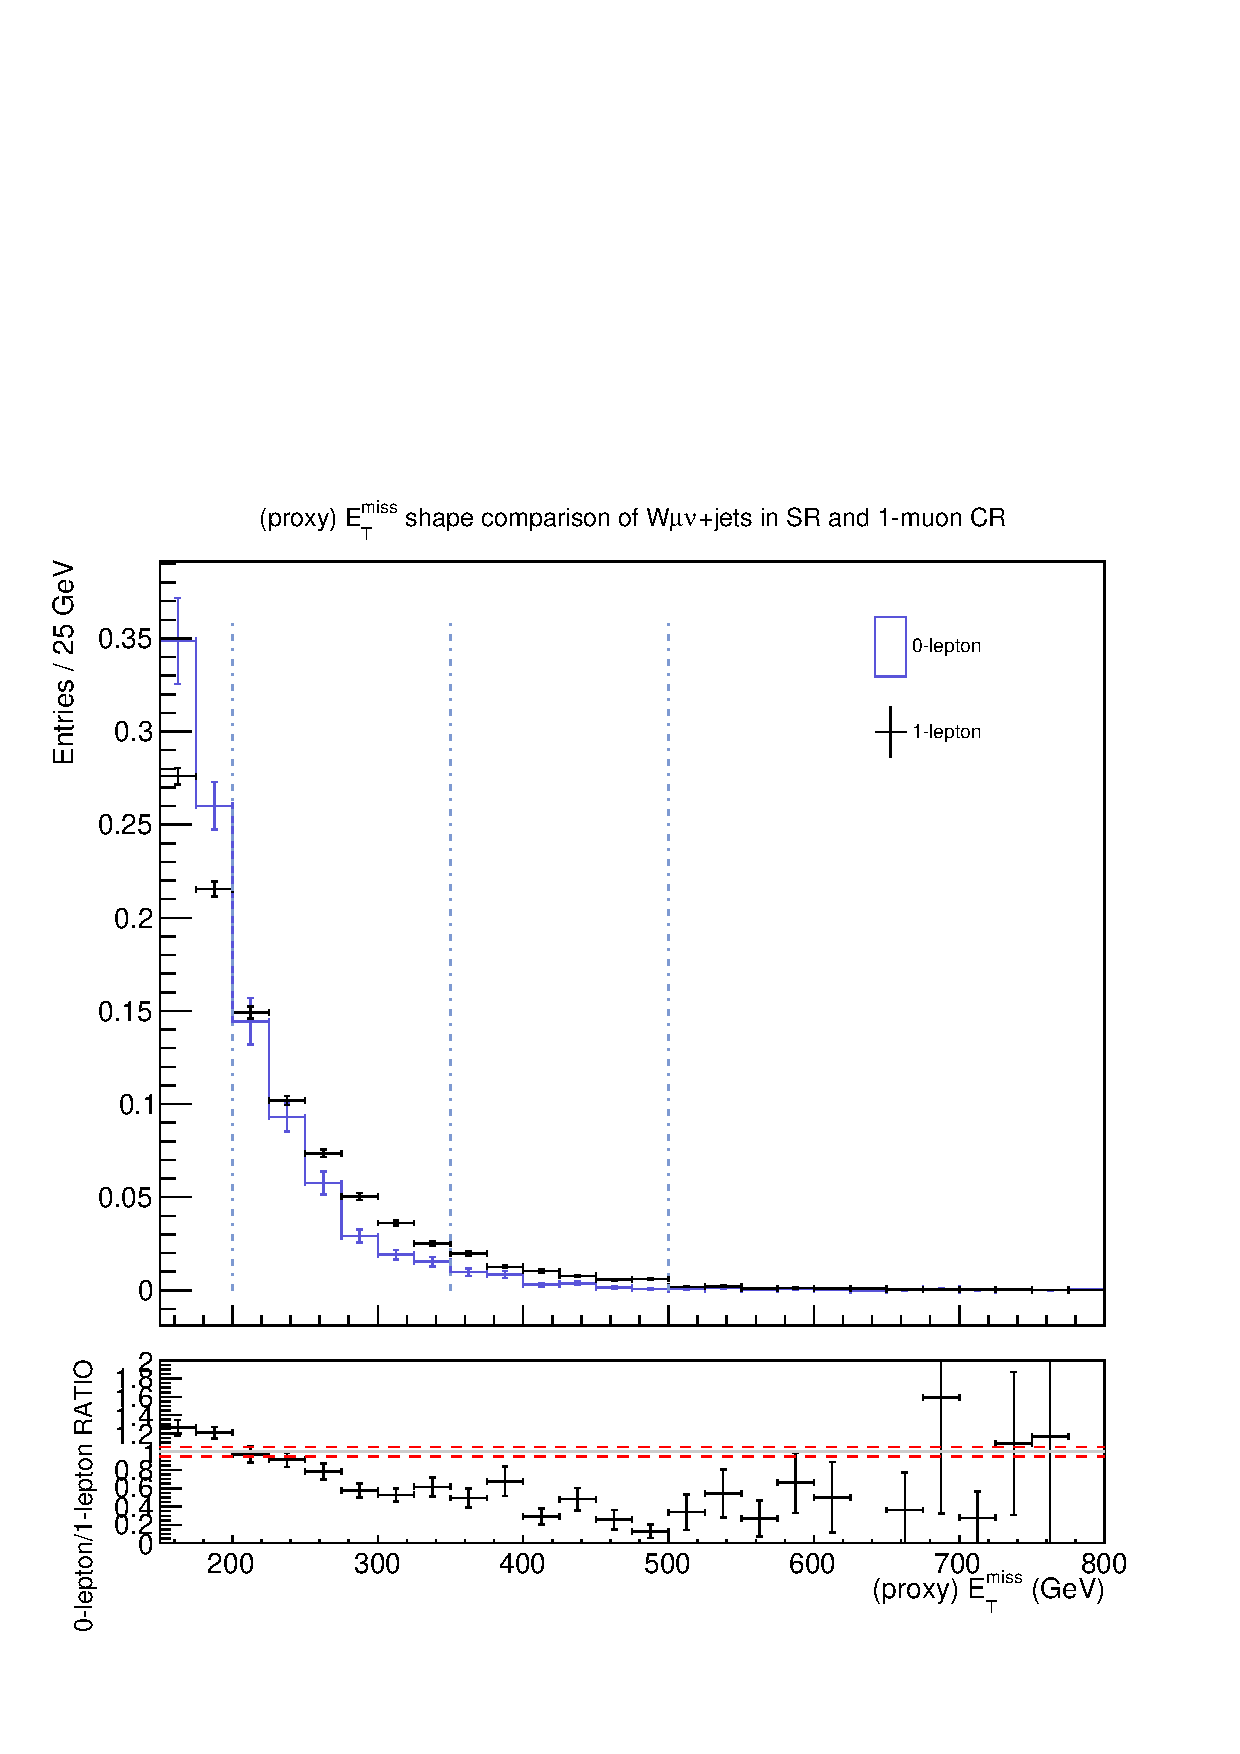
\includegraphics[width=0.45\linewidth]{manybins.pdf}}
		%	~
			%\vspace{\baselineskip}
		%	\subcaptionbox
		%	{\label{fig:subfig_twoPTV}}
		%	{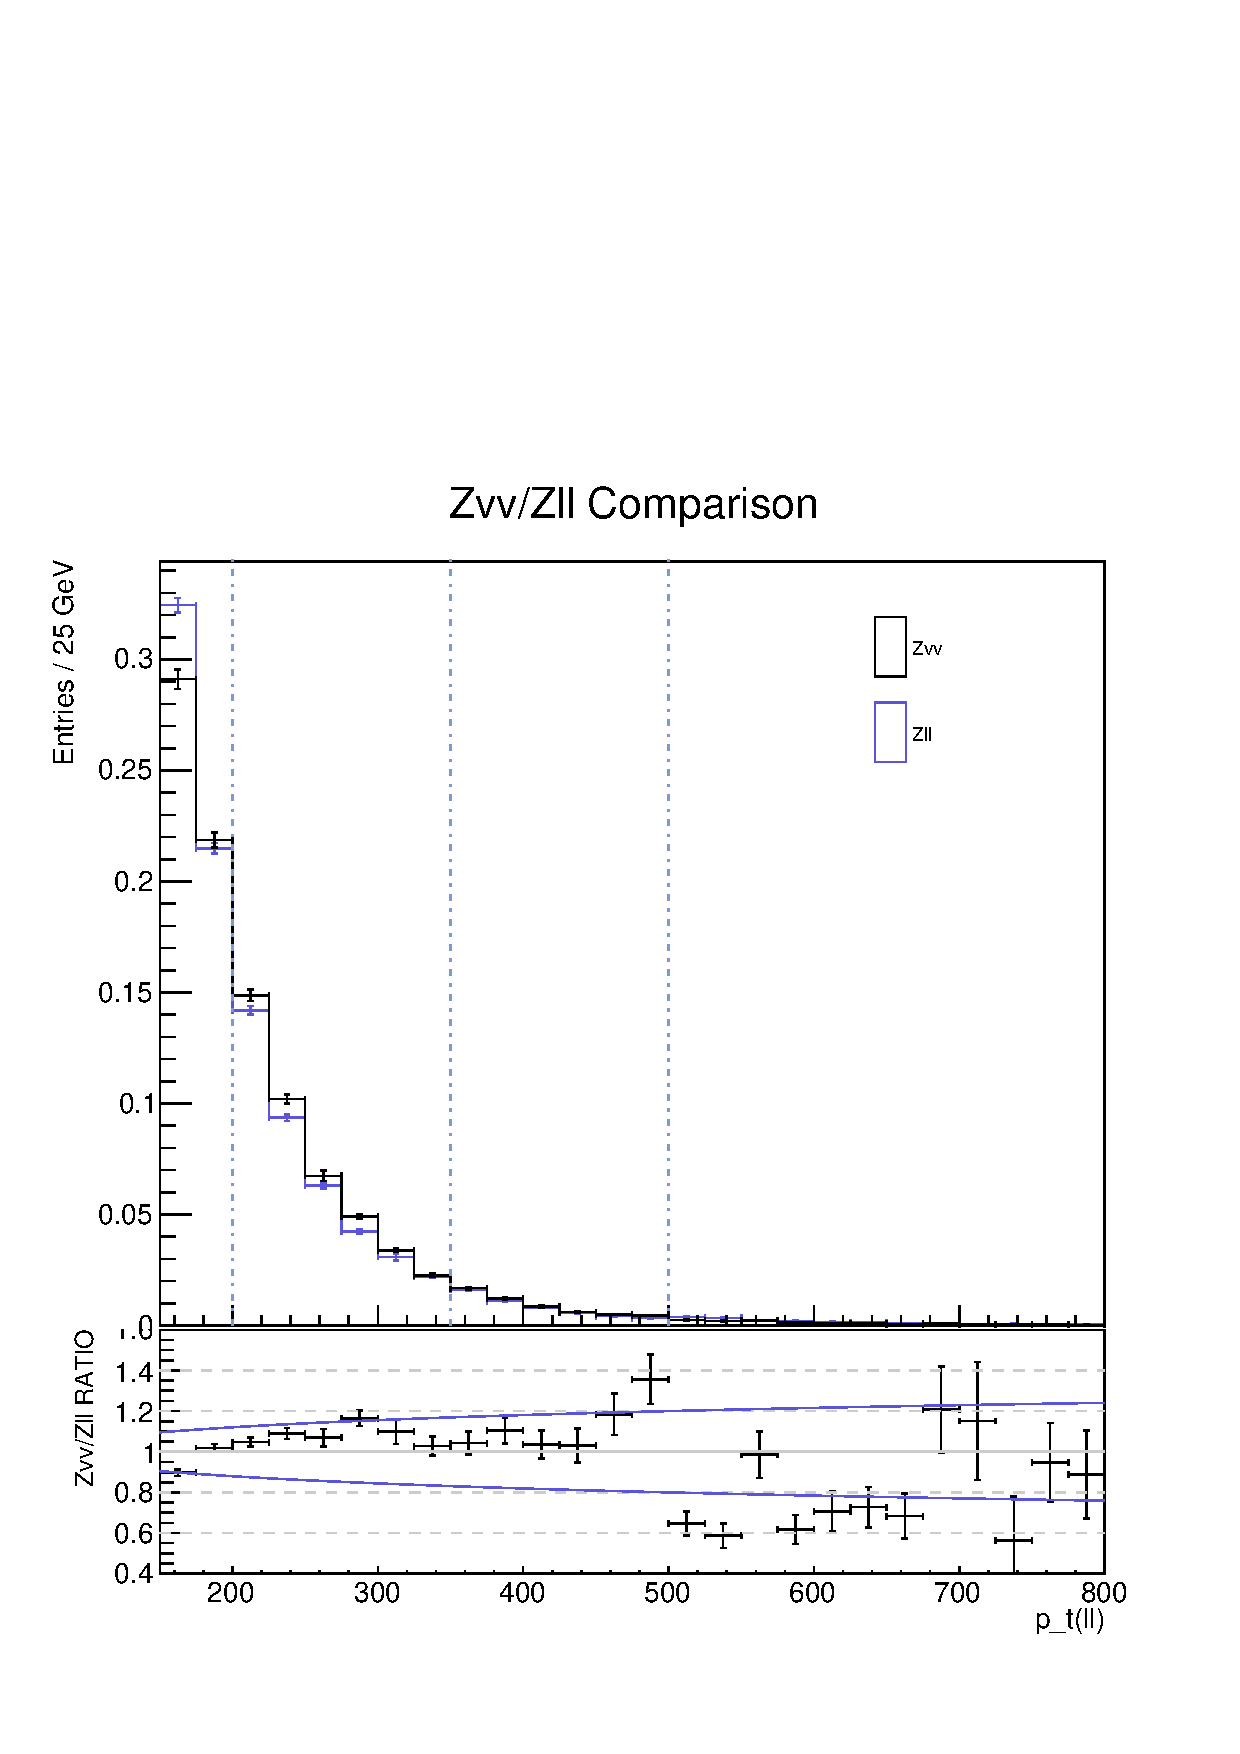
\includegraphics[width=0.45\linewidth]{twoMET.pdf}}
		%	\caption{\subref{fig:subfig_onePTV}The comparison of the (proxy) $E_T^{\mathrm{miss}}$ between SR and one-muon CR for the W($\mu \nu$)+jets events. \subref{fig:subfig_twoPTV}The compasion of the (proxy) $E_T^{\mathrm{miss}}$ between SR and two-lepton CR for the Z+jets events. Both the upper pannels show the normalized distribution and the lower pannels show the ratio of SR to CRs. The latter plot is meant to be an approximation to how large the ratio of the former plot is.}
		%	\label{fig:MET_comparison}
		%\end{figure}
	
		%\fig[0.5][fig:mjj_distribution][!hbt]{mjj_distribution.pdf}[The dijet mass distribution comparison of W($\mu \nu)$+jets in SR and one-muon CR. The upper pannel shows the distribution after normalization. The lower pannel shows the ratio of the yields in SR to one-muon CR.][short caption]
		
		From figure \ref{fig:MET_comparison}, two interseting things are found. First, the shape distribution has the same trend. Second, the ratios between the SR and one-muon CR are generally away from the 5\% difference as shown.  It is noticed that at lower energy, the ratios are larger than the upper limit and, at higher energy, the ratios are less than the lower limit, except for the last few bins, where the statistics are low. That is to say, at lower energy, W($\mu \nu$)+jets events underestimate the backgrounds in SR, and at higher energy, overestimation happens.
		
		In author's opinion, although the W($\mu \nu$)+jets events are the same in both SR and one-muon CR, the situation is a little bit different. These events would appear in the SR only when the muon is misidentified. If the muon is soft, which means it has low $p_T$, it's more likely to be misidentified and thus be reconstructed as $E_T^{\mathrm{miss}}$. On the other hand, if the $p_T$ is higher, misidentification are less likely to happen and the muon are rejected by the selection of SR. Therefore, more events whose muons have higher $p_T$ are removed in the SR but events with more low $p_T$ muons stay in the SR. This means that the true simulation, which is expected in one-muon CR, underestimates the yields at lower energy and overestimate at higher energy. Due to this poor estimation, one sees the severely flucuating ratio values.
		
		As a minor conclusion, the W($\mu \nu$)+jets comparison between SR and CR doesn't quite fit in the 5\% limit. One of the assumption on this is that the over- and under- estimation on different value of $p_T$ are not well covered by the uncertainty. The yield uncertainty shall be recalculated for this issue.

\chapter{Results of monoHbb Analysis}

\section{Main Uncertainties}
	The systematic uncertainties dominate the main uncertainty in this analysis. Among them, the b-tagging efficiency, the integrated luminosity, jet energy scale (JES) and jet energy resolution (JER) contribute the most to the experimental uncertainty. The SM predictions are the sources of the theoretical uncertainties. $t\bar{t}$ events, W/Z +jets events, associated production of SM Higgs boson decay into $b\bar{b}$ (Vh($b\bar{b}$), where V is the vector boson) and diboson events dominate the theoretical uncertainties.
	
	The uncertainty on the b-tagging efficiency originate from the flavor tagging efficiency in the $t\bar{t}$ events. A calibration, which highly makes use of beam testing in LHC, on the integrated luminosity is performed with a value a 2.0\%.
	
	The theoretical uncertainties originate from the SM modeling. Normalizations, acceptance difference and differential distributions of important kinematic variables derive the uncertainties.
	
\section{Results}
	A fit to the invariant mass of Higgs candidate $m_h$ is used to search for the signal. For resolved region, $m_{\mathrm{jj}}$ represents the Higgs mass while $m_{\mathrm{J}}$ is used in the merged region.
	
	The fit is based on a likelihood based approach. The systematic uncertainties are used in the likelihood function as nuisance parameters. The data in SR and two CRs are fit simultaneously for all four different (proxy) $E_T^{\mathrm{miss}}$ bins: $\left[150, 200\right)$ GeV, $\left[200, 350\right)$ GeV, $\left[350, 500\right)$ GeV, and $\left[500, \infty \right)$ GeV. $m_h$ is the fit variable in the SR. The fit variable used in the one-muon CR is the $\mu$ lepton charge. $t\bar{t}$ processes tend to produce the same amount of $\mu^+$ and $\mu^-$ leptons but the W+jets events produce more $\mu^+$ than $\mu^-$ leptons, which originates from proton-proton collision in LHC and from the conservation of electric charge. $\mu$-charge can thus be made use of as a differentiation of $t\bar{t}$ and W+jets events. In the two-lepton CR, the event yields serve as the fit variable because of limited data statistics.
	
	Figure \ref{fig:MET_SR} shows the $E_T^{\mathrm{miss}}$ distribution in SR. Figure \ref{fig:SR_mj} shows the distribution of $m_{\mathrm{jj}}$ or $m_{\mathrm{J}}$ in SR for resolved and merged region respectively. The data yields agree with the SM predictions. That is to say, no significant excess of the signal is found.
	
	An exclusion limit at 95\% confidence level (CL) is used for the interpretation of this analysis. The exclusion contour in $(m_{\mathrm{A}}, m_{\mathrm{Z'}})$ phase space is shown in figure \ref{fig:exclusion}. It also shows the result in the previous iteration. As it suggests, more region are excluded compared to the previous result. Figure \ref{fig:signal strength} shows the comparison of the upper limit of the signal strength between this result and the previous result, in which the fixed-radius (FR) track jets are used. In contrast to VR, FR track jets have a fixed cone size of $R = 0.2$. The plot also suggests more region in the phase space is excluded.
	
	\fig[0.6][fig:MET_SR][!hbt]{MET_SR.png}[The $E_T^{\mathrm{miss}}$ distribution for resolved and merged combined in SR. The dashed blue lines are the expectation yields before fits. The solid histograms are the simulations after fit. The dashed red lines are the expected signal from Z'-2HDM model.][short caption]
	
	\begin{figure}[!hbt]
		%\captionsetup[subfigure]{labelformat=empty} % hide figure's number.
		\centering
		\subcaptionbox
		{\label{fig:subfig_SR_mjj_150_200}}
		{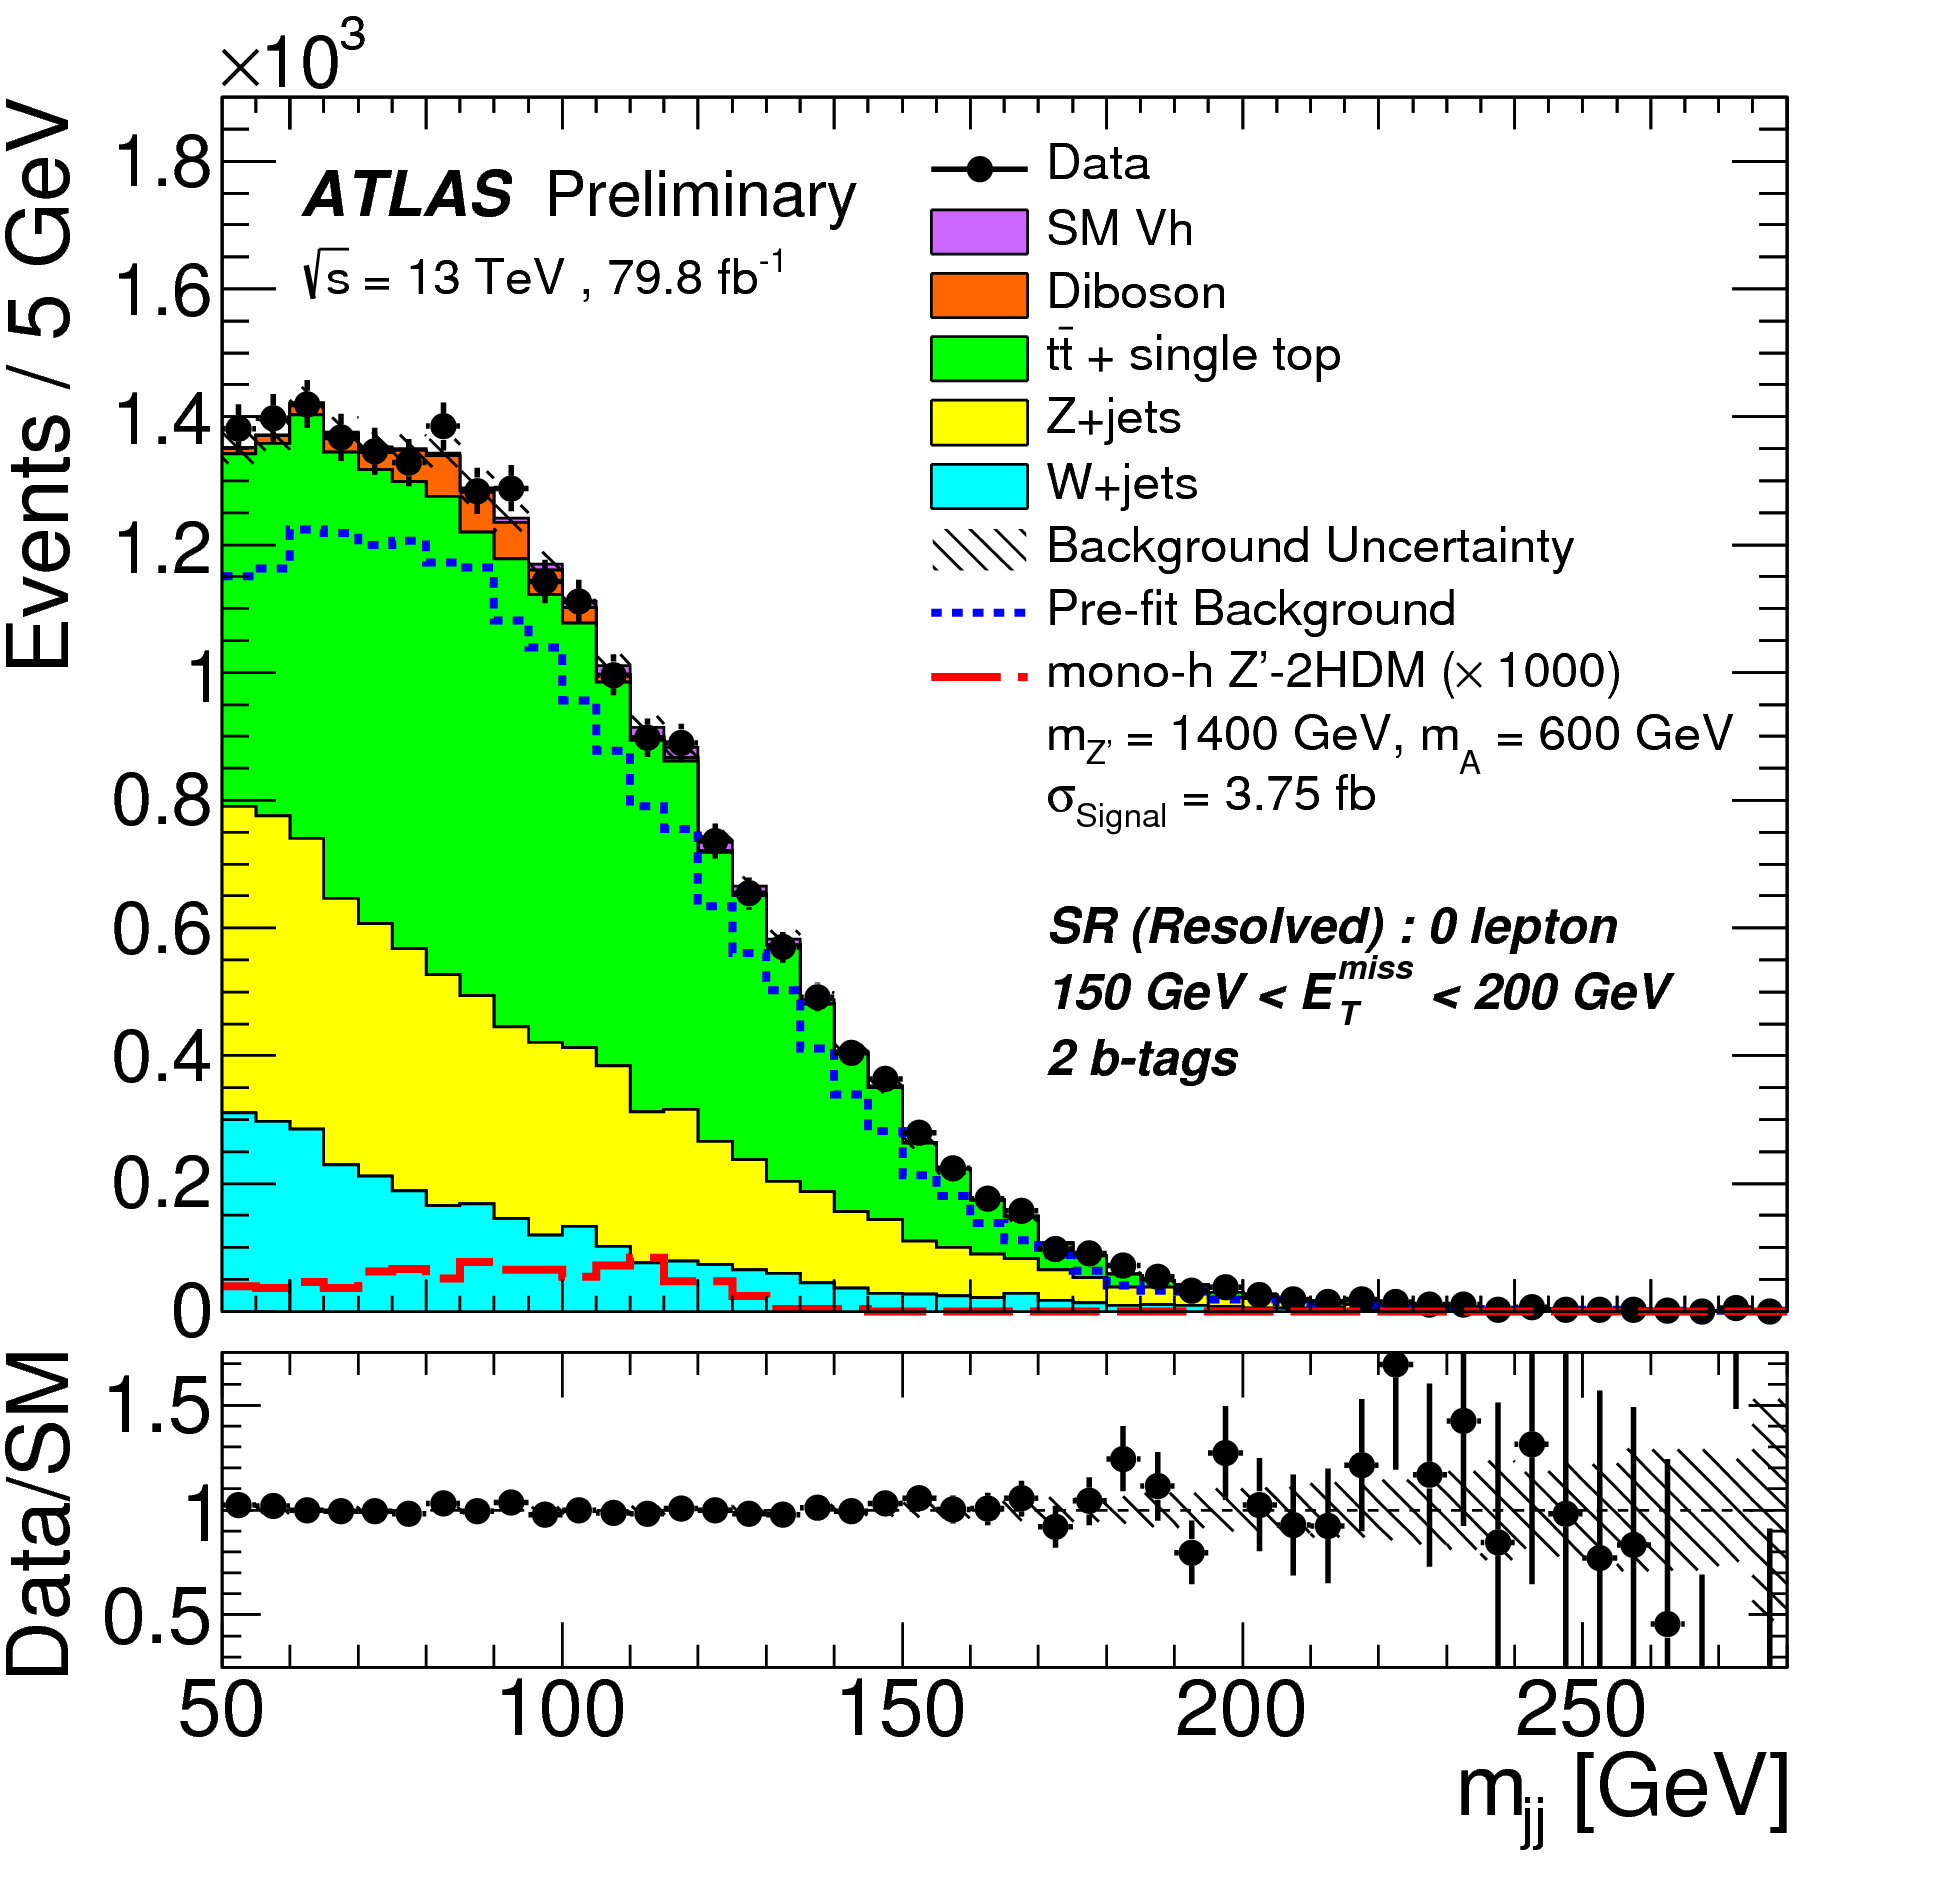
\includegraphics[width=0.4\linewidth]{SR_mjj_150_200.png}}
		~
		\subcaptionbox
		{\label{fig:subfig_SR_mjj_200_350}}
		{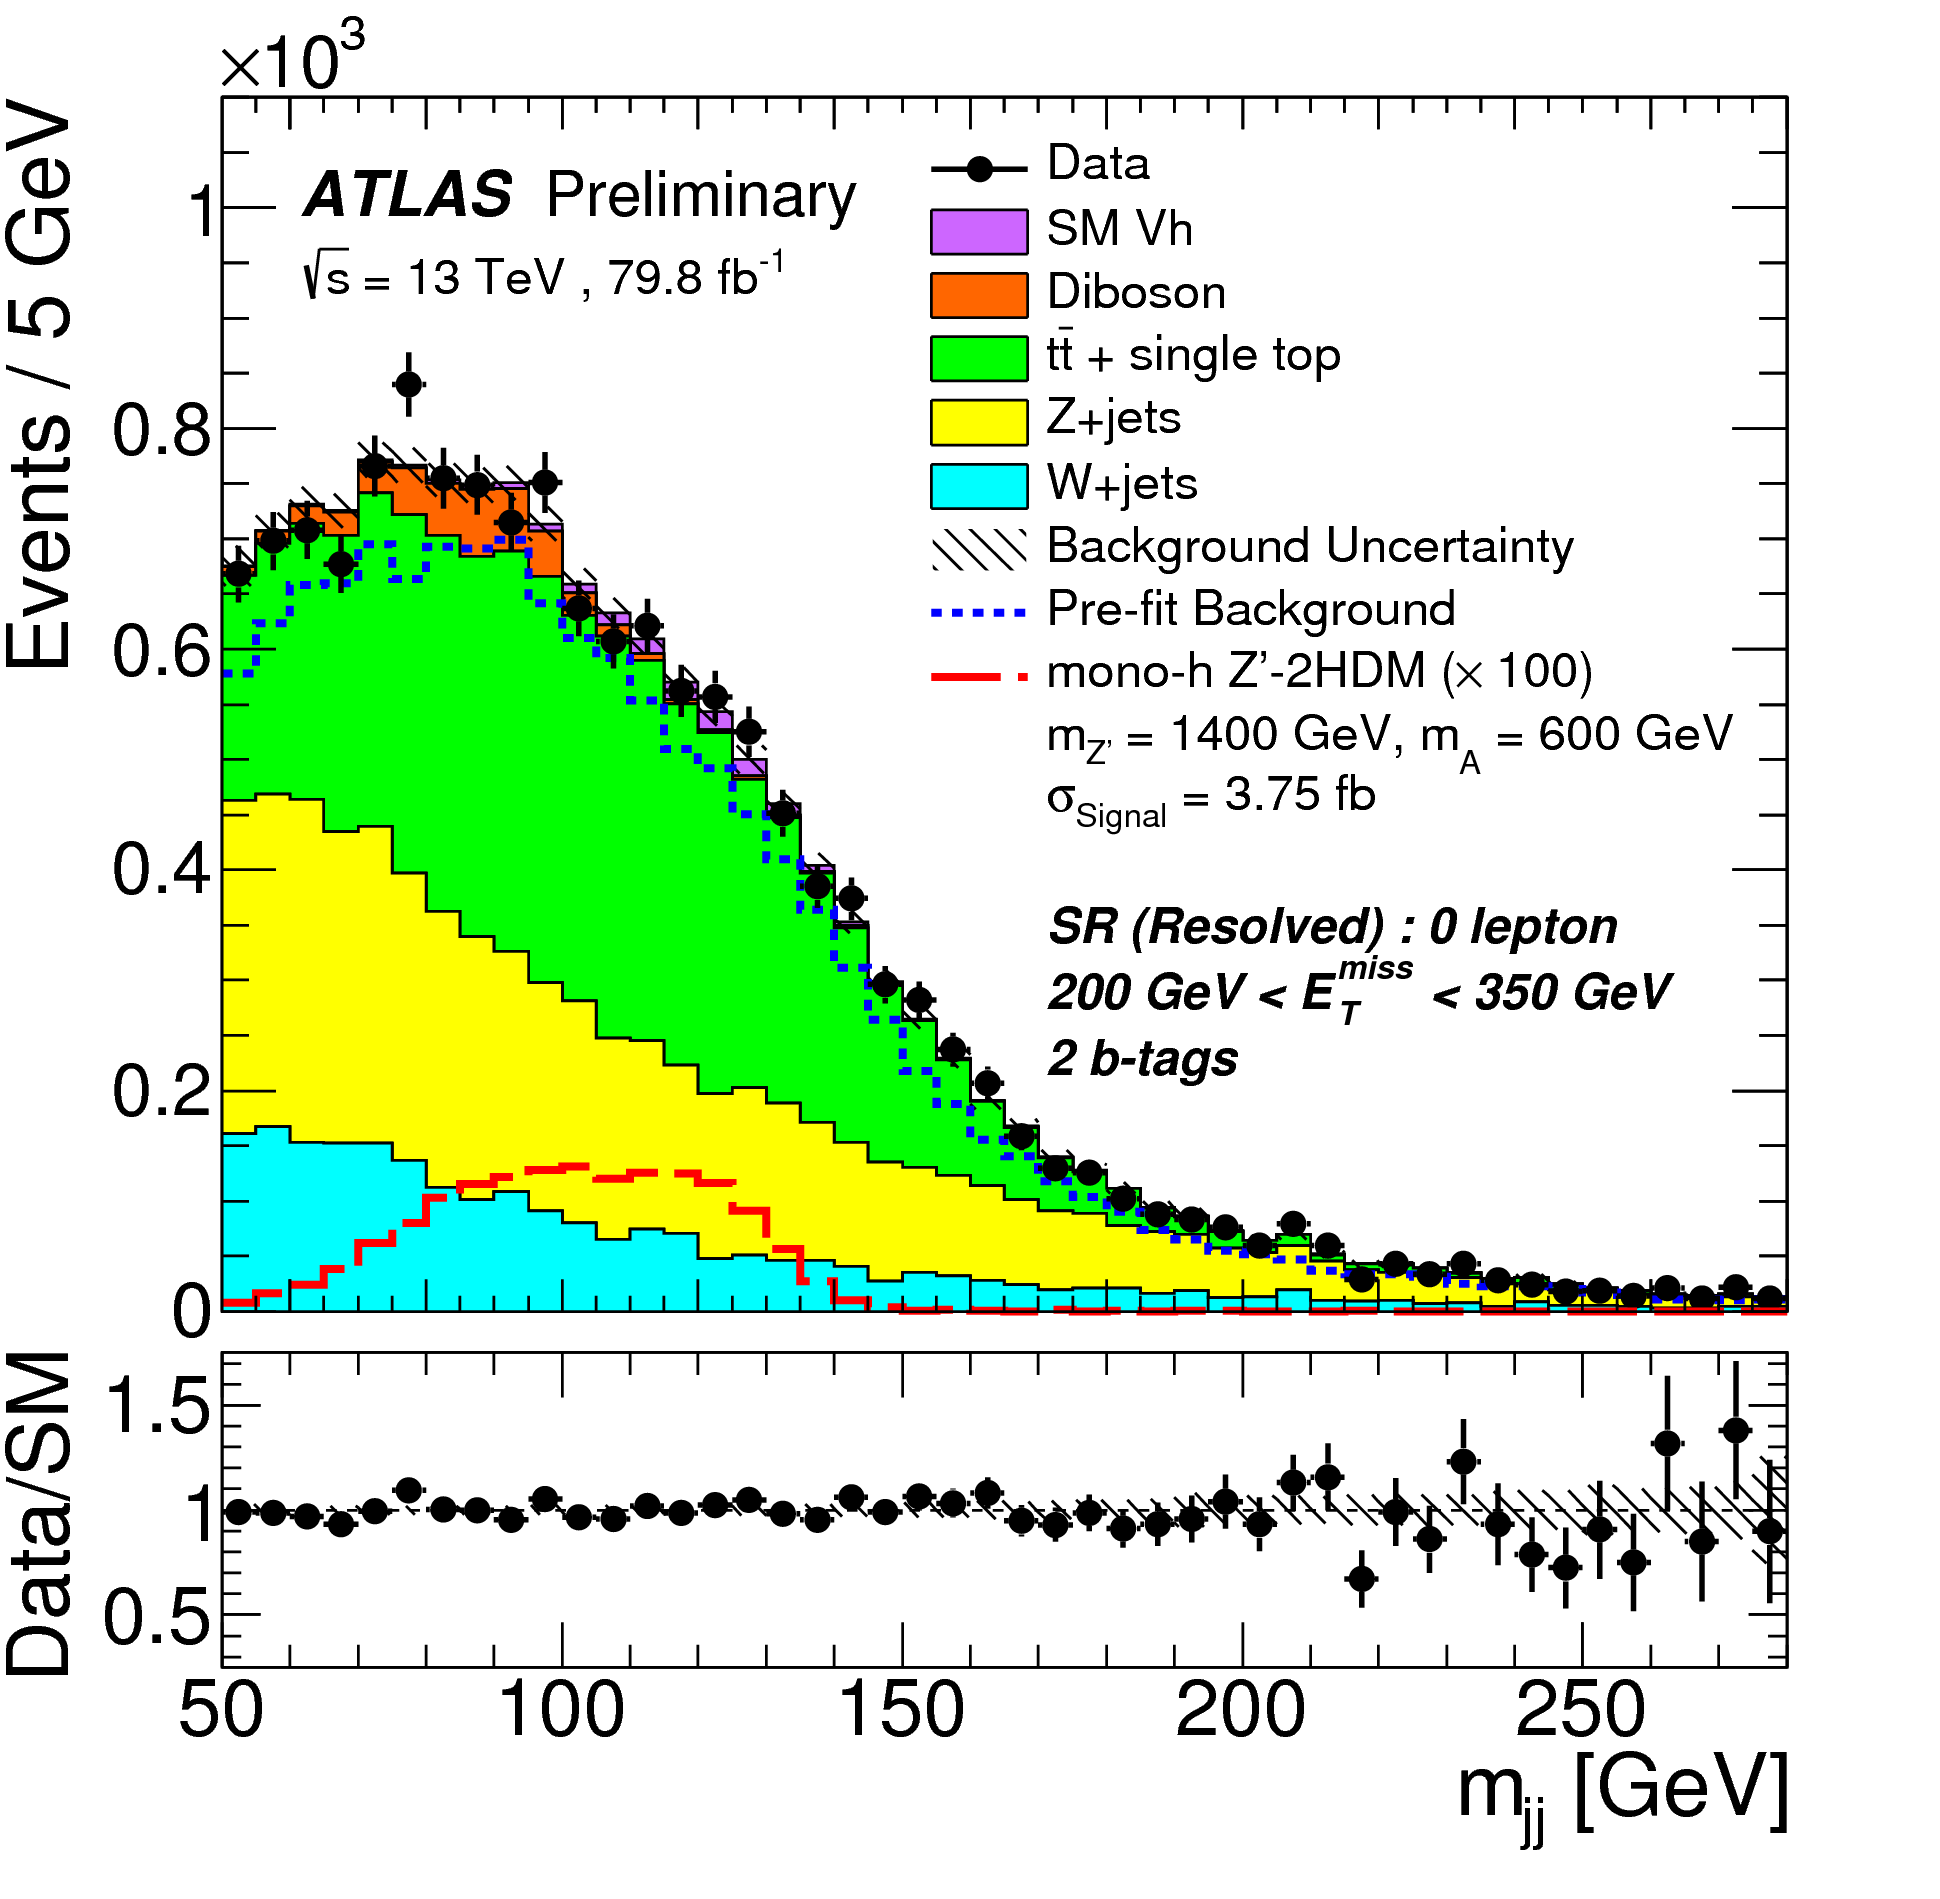
\includegraphics[width=0.4\linewidth]{SR_mjj_200_350.png}}
		\vspace{\baselineskip} % 分隔上下列
		\subcaptionbox
		{\label{fig:subfig_SR_mjj_350_500}}
		{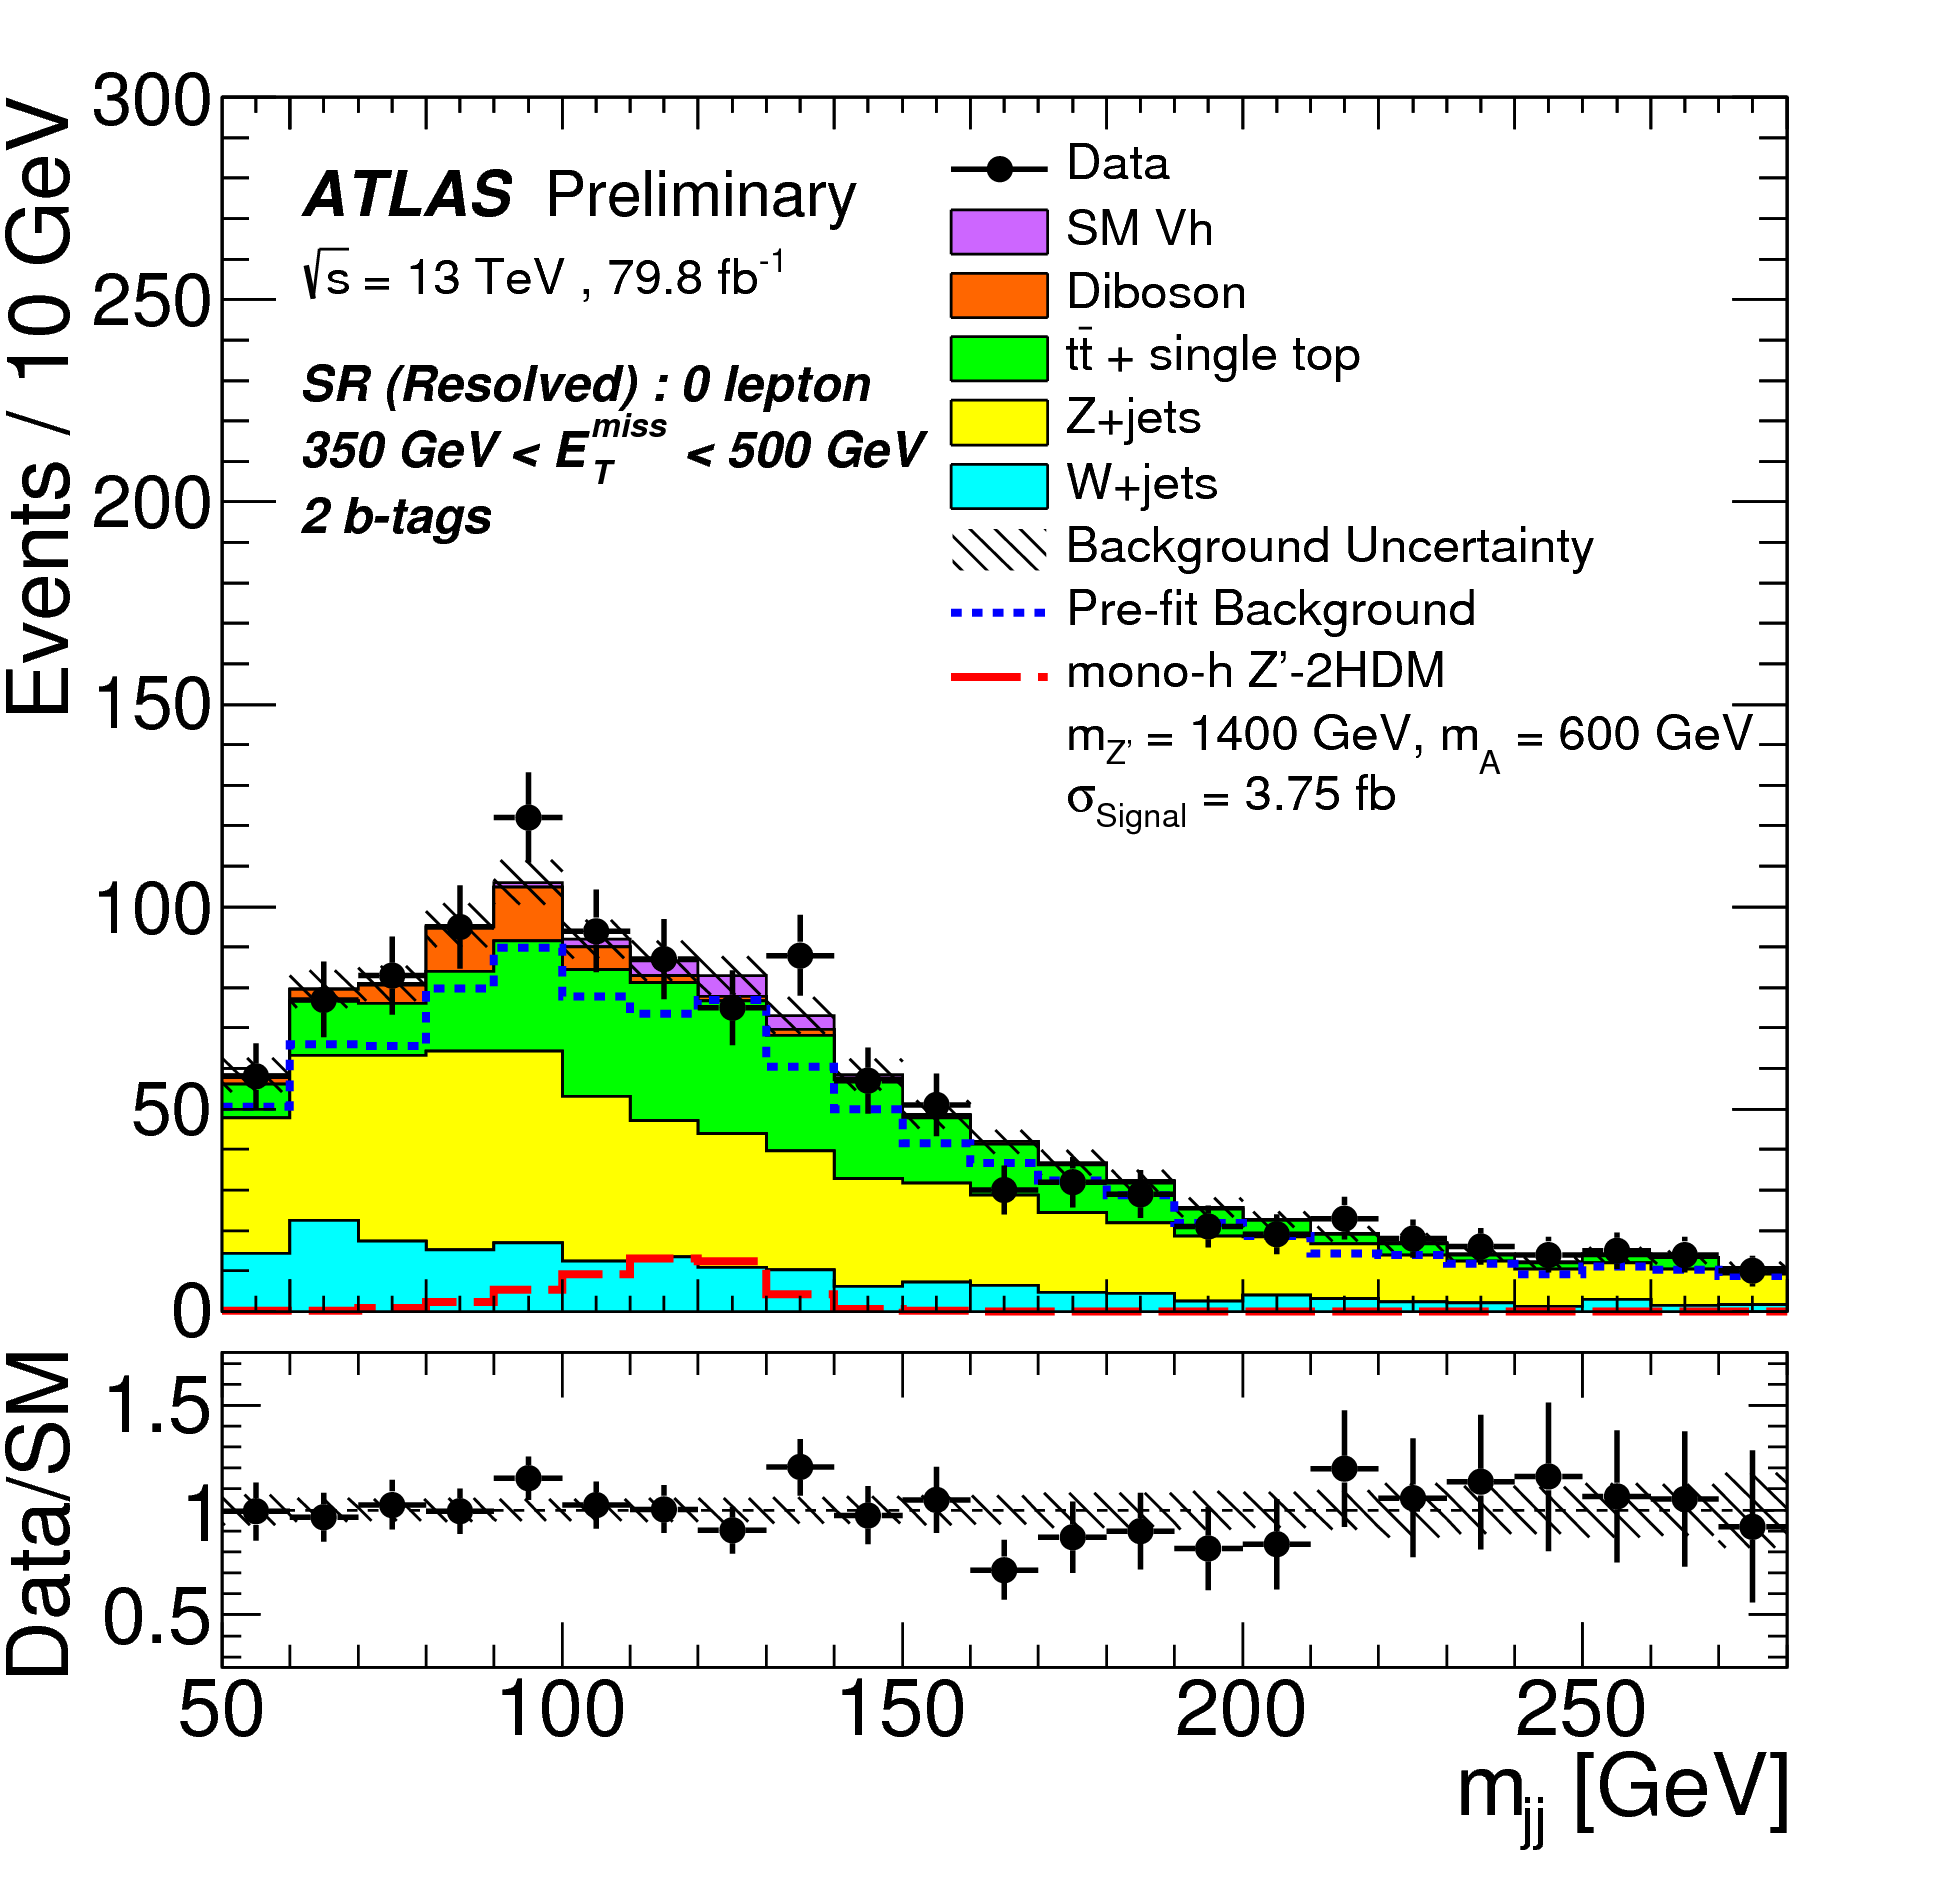
\includegraphics[width=0.4\linewidth]{SR_mjj_350_500.png}}
		\subcaptionbox
		{\label{fig:subfig_SR_mJ_500}}
		{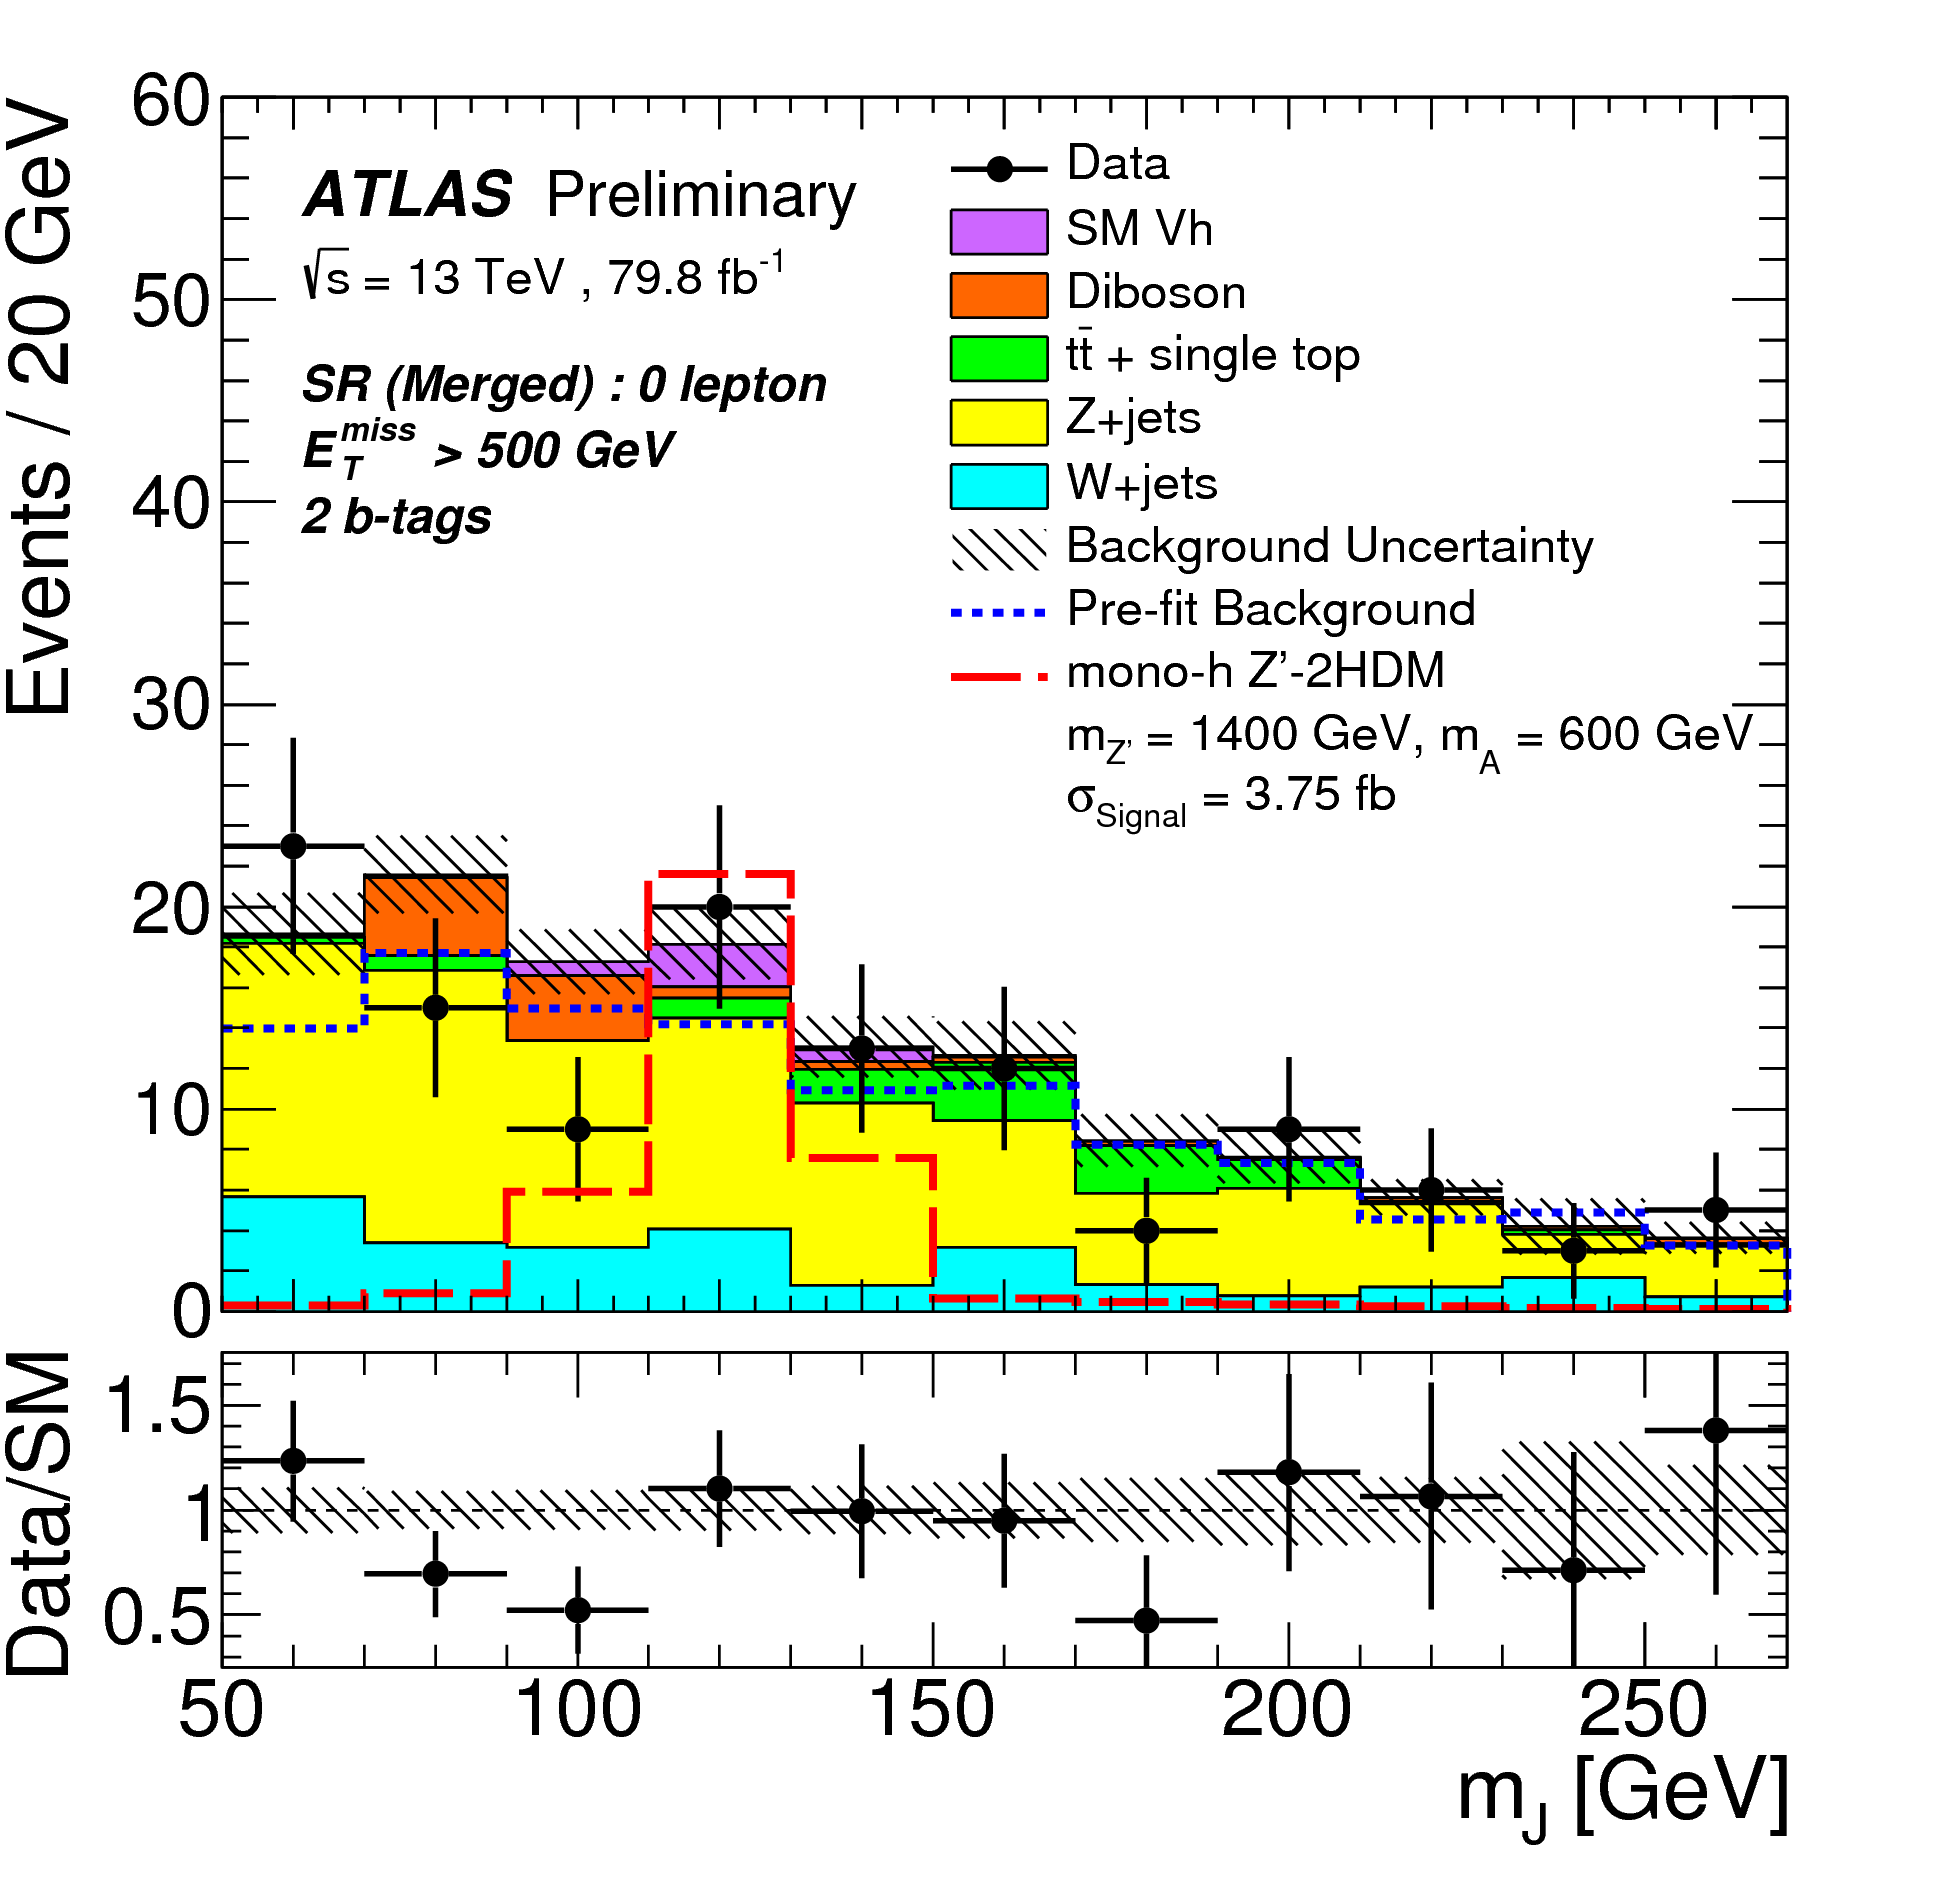
\includegraphics[width=0.4\linewidth]{SR_mJ_500.png}}
		\caption{Distirbution of the invariant mass of the Higgs boson candidate $m_{\mathrm{h}}$ with two b-tagged jets. The upper two plots are for $E_T^{\mathrm{miss}} \in \left[150, 200\right)$ GeV and $\left[200, 350\right)$ GeV bins. The lower two ones are for $E_T^{\mathrm{miss}} \in \left[350, 500\right)$ GeV and $\left[500, \infty \right)$ GeV. The dashed blue lines are the expectation yields before fits. The solid histograms are the simulations after fits. The dashed red lines are the expected signal from Z'-2HDM model. Its yields for the upper two plots are scaled up by a factor of 100 and 1000 from left to right respectively.}
		\label{fig:SR_mj}
	\end{figure}
	
	\fig[0.6][fig:exclusion][!hbt]{exclusion.png}[Exclusion contour in $(m_{\mathrm{A}}, m_{\mathrm{Z'}})$ phase space. Regions under the curve are excluded. The solid line shows consistency with SM-only hypothesis. The dashed blue line are the results from previous ATLAS results of $\sqrt{s} = 13$ TeV.][short caption]
	
	\fig[0.6][fig:signal strength][!hbt]{signal_strength.png}[The upper limit of the signal strength of this model with $m_{\mathrm{A}}$ fixed at 500 GeV. The dashed red line is the result of previous iteration, which made use of FR track jets. The dashed black line in the result of this iteration, where VR track jets are used. Signals, if exist, would appear in the region where the signal strength is greater than one. As a result, all regions whose upper limit is smaller than one is excluded. As the plot shows, making use of VR track jets extends the excluded region.][short caption]


\chapter{Conclusion}\label{result}
	To sum up, a collider search for the dark matter in association with a final state of $E_T^{\mathrm{miss}}$ and $b\bar{b}$, which decay from the Higgs boson candidate, was performed using 79.8 $fb^{-1}$ of proton-proton collision at $\sqrt{s} = 13$ TeV recorded in the ATLAS at LHC. The results are in agreement with SM predictions. An exclusion on the parameter space of Z'-2HDM model is excluded, up to $m_{\mathrm{Z'}} = 2.8$ TeV and $m_{\mathrm{A}} = 300$ GeV.

\end{document}
    \backmatter          % book class 預設\backmatter 在\appendix 後面。因此.cls修改過\appendix 定義
        % This file has 3 types bibliography management, 
% \bibManType in config.tex choose it.
% 0. Embedded: write \bibitem in {thebibliography} environment.
% 1. BibTeX: Change bib files in \bibliography{}
% 2. biber / BibLaTeX: Add bibliography by \addbibresource{bibfile.bib} in macros_preamble.tex

\documentclass[class=NCU_thesis, crop=false]{standalone}

\begin{document}

\ifcase \bibManType 
    % 0 == Embedded %%%%%%%%%%%%%%%%%%%%%%%%%%%%%%%%%%%%%%%
    {\bibFontStyle\setstretch{\bibLineStretch}
    \begin{thebibliography}{99}

    \bibitem{cite_key_1}
        bibliography item detail.

    \bibitem{_sppmg/tw_thesis_template_????}
        TW\_Thesis\_Template,
        sppmg,
        \url{https://github.com/sppmg/TW_Thesis_Template},
        Embedded bibliography demo.

    \end{thebibliography}
    }
    
\or
    % 1 == BibTeX %%%%%%%%%%%%%%%%%%%%%%%%%%%%%%%%%%%%%%%%%
    \bibliographystyle{\bibStyle}
    {\bibFontStyle\setstretch{\bibLineStretch}
        \bibliography{demo} % {sample_1,sample_2,...,sample_n}
        % Note the lack of whitespace between the commas and the next bib file.
    }
\or

    % 2 == biber / BibLaTeX %%%%%%%%%%%%%%%%%%%%%%%%%%%%%%%
    \printbibliography[heading = bibnumbered]
\fi



\end{document}
    \appendix
        \documentclass[class=NCU_thesis, crop=false]{standalone}
\begin{document}

\chapter{List of device}

\begin{table}[!h]
    \centering
    \begin{tabularx}{\textwidth}{|l|l|X|}
        \hline
        device  & Model    & Description \\ \hline
        Linux   & Debian 9 & Best of best of best OS \\ \hline
        Windows & 10       & Best of Best tool to prevent the aging of brain. \\ \hline
    \end{tabularx}
    \caption{List of device}
    \label{table:list_device}
\end{table}

\end{document}
        \documentclass[class=NCU_thesis, crop=false]{standalone}
\begin{document}

\definecolor{Gray3}{gray}{0.8}

\chapter{Solutions}

\section{The solution}
\begin{table}[!h]
    \centering
    \begin{tabular}{| l | l |}
        \hline
        Component & Concentration(mM) \\ \hline
        \rowcolor{Gray3}
        \ce{NaCl} & 1.0 \\ \hline
        \ce{CaCl_2} & 2.0 \\ \hline
        \rowcolor{Gray3}
        \ce{NaCl} & 1.0 \\ \hline
        \ce{CaCl_2} & 2.0 \\ \hline
    \end{tabular}
    \caption{The solution}
\end{table}
\end{document}
        \documentclass[class=NCU_thesis, crop=false]{standalone}
\begin{document}
% Here demo instert whole code file. You can only insert code directly, 
% please read my tutorial or document of listings package.
% code style set in macros_preamble already.
% Supported language please read document of listings package.


\chapter{Code}
\section{C}
\lstinputlisting[language=C]{hello_world_c.c}

\section{Matlab}
\lstinputlisting[language=matlab]{hello_world_matlab.m}

\section{IDL}
\lstinputlisting[language=IDL]{hello_world_idl.pro}
\end{document}

%         \documentclass[class=NCU_thesis, crop=false]{standalone}

\begin{document}
\chapter{Letters bot}

Here try to insert some information automatically.
If you need change font size or position, modify appendix\_letter\_NCU.tex and compile this single tex file.

In appendix\_letter\_NCU.tex, you will see \textbackslash{}placetextbox for every string.
\begin{lstlisting}[style=LatexStyle,caption={}]
\placetextbox{x(mm)}{y(mm)}
\end{lstlisting}

The unit is mm , origin at bottom left. I recommend add ``colorgrid'' option to ``\textbackslash{}documentclass'' for positioning. e.g. In this tex file (appendix\_letter\_NCU.tex):

\begin{lstlisting}[style=LatexStyle,caption={}]
\documentclass[class=NCU_thesis, crop=false, colorgrid]{standalone}
\end{lstlisting}

``colorgrid'' will display a grid with mm unit. 

\begin{center}
{ \noindent\color{red}\bfseries\Large NCU 中文文件位於 NCU\_zh}
\end{center}

%%%%%%%%%%%%%%%%%%%%%%%%%%%%%%%%
% define \mprof 
\ExplSyntaxOn
    % Copy prof. list from config.tex
    \clist_gclear_new:N \g_sppmg_profs_cl
    \clist_gset:NV \g_sppmg_profs_cl \profs
    \clist_gpop:NNTF \g_sppmg_profs_cl \l_tmpa_tl {}{ \tl_clear:N \l_tmpa_tl}
    \cs_gset_eq:NN \mprof \l_tmpa_tl
\ExplSyntaxOff

% Define local variable (e.g. cover use \titleZh for \title but letters use \titleEn )
\def\title{\titleEn}

%%%%%%%%%%%%%%%%%%%%%%%%%%%%%%%%
\cleardoublepage
\pagestyle{empty}
\sffamily
% ------------------------------

% 碩博士論文電子檔授權書
\IfFileExists{\letterAuthEl}{
\cleardoublepage\thispagestyle{empty}
\includepdf[pagecommand={   \placetextbox{115}{87}{\fs{14}\title}%
                            \placetextbox{100}{81}{\fs{14}\mprof}%
                            \placetextbox{85}{70}{\fs{14}\deptshort} }]%
{\letterAuthEl}}{}

% 碩博士紙本論文延後公開/下架申請書。(如需延後公開者,才需要裝訂於論文內頁)
\IfFileExists{\letterPubReq}{
\cleardoublepage\thispagestyle{empty}
\includepdf[pagecommand={   \placetextbox{128}{269}{\fs{14}\author}%
                            \placetextbox{70}{255}{\fs{14}\deptshort}%
                            \placetextbox{100}{231}{\fs{14}\title}%
                            \placetextbox{90}{218.3}{\fs{14}\mprof} }]%
{\letterPubReq}}{}

% 指導教授推薦書
\IfFileExists{\letterRecom}{
\cleardoublepage\thispagestyle{empty}
\includepdf[pagecommand={   \placetextbox{75}{204}{\fs{16}\deptshort}%
                            \placetextbox{90}{218}{\fs{16}\author}%
                            \placetextbox{105}{192}{\fs{16}\title}}%
]{\letterRecom}}{}

% 口試委員審定書
\IfFileExists{\letterVerif}{
\cleardoublepage\thispagestyle{empty}
\includepdf[pagecommand={   \placetextbox{75}{184}{\fs{16}\deptshort}%
                            \placetextbox{91}{200}{\fs{16}\author}%
                            \placetextbox{100}{170}{\fs{16}\title}}%
]{\letterVerif}}{}

% ------------------------------
\pagestyle{fancy}
\end{document}
\end{document}